\documentclass[12pt,a4paper,twoside,openright]{report}
\usepackage{algpseudocode}		% ambienti per la scrittura di algoritmi
\usepackage{algorithm}			% 

\usepackage{pifont}						% http://ctan.org/pkg/pifont
\usepackage{epsfig}						% figure eps
\usepackage{graphicx}					% figure qualsiasi
\usepackage{amsmath,amsfonts,amsthm}		% package di scrittura matematica
\usepackage{amssymb}
\usepackage{psfrag}
\usepackage{fancyhdr}
\usepackage{url}
\usepackage{array}
\usepackage{subfigure}
\usepackage{lscape}
\usepackage{colortbl}
\usepackage{alltt}
\usepackage{tabularx}
\usepackage[english]{babel}
\usepackage[nottoc]{tocbibind}
\sloppy
\raggedbottom

\linespread{1.3}
\renewcommand{\baselinestretch}{1.3}

\makeatletter
\def\cleardoublepage{\clearpage\if@twoside \ifodd\c@page\else
\hbox{}
\vspace*{\fill}
\begin{center}
%This page intentionally contains only this sentence.
\end{center}
\vspace{\fill}
\thispagestyle{empty}
\newpage
\if@twocolumn\hbox{}\newpage\fi\fi\fi}
\makeatother

%\newcites{wb}{Web References}

%------------------------------------------------------
% Impostazioni per il controllo sillabazione vedove/orfane ect..
%
% \looseness=1 o \looseness=-1 prima di un paragrafo per
% allungarlo o accorciarlo di una riga
%------------------------------------------------------

\lefthyphenmin=4
\righthyphenmin=4
\tolerance=1000
\hyphenpenalty=100
\emergencystretch=1 cm

\widowpenalty=5000
\clubpenalty=2500

%--------------------------------------------------------
% impostazioni per la dimensione delle pagine
%--------------------------------------------------------
\renewcommand{\headrulewidth}{0.5pt}
\hoffset=-15mm
%\topmargin=0mm
\headheight=15pt
\textwidth=140mm
\headsep=5mm
\voffset=-5mm
%\hsize=13cm
%\textwidth=164mm
\textheight=230mm
\evensidemargin=25mm
\oddsidemargin=25mm
%\marginparwidth=0mm

\renewcommand{\abovecaptionskip}{0pt}
\renewcommand{\belowcaptionskip}{0pt}

%--------------------------------------------------------------
% impostazione headers
%--------------------------------------------------------------
\pagestyle{fancy}
%\addtolength{\headwidth}{\marginparsep}
%\addtolength{\headwidth}{\marginparwidth}
\renewcommand{\chaptermark}[1]{\markboth{#1}{}}
\renewcommand{\sectionmark}[1]{\markright{\thesection\ #1}}
\fancyhf{}
\fancyfoot[LE,RO]{\bfseries\thepage}
\fancyhead[RO]{\bfseries\rightmark}
\fancyhead[LE]{\bfseries\leftmark}
\fancypagestyle{plain}{%
\fancyhead{} % get rid of headers
\fancyfoot{}
\renewcommand{\headrulewidth}{0pt} % and the line
}

\newenvironment{myverse}
{\small}
{}

\newenvironment{myabstract}{%
  \begin{center}%
    \null\vfil
    \bfseries \abstractname
  \end{center}}%
{\par\vfil\null}

%--------------------------------------------------------------------------------
% custom commands %--------------------------------------------------------------------------------
\newcommand{\newparagraph}{\noindent\\}
\newcommand{\xmark}{\ding{55}}
\newcommand{\cmark}{\ding{51}}

%--------------------------------------------------------------------------------
% document start
%--------------------------------------------------------------------------------
\begin{document}

\pagenumbering{roman}
\setcounter{page}{1}
\pagestyle{empty}

%--------------------------------------------------------------------------------
% include title page
%--------------------------------------------------------------------------------
\begin{titlepage}
\vspace*{-2.5cm}
\bfseries

\begin{center}
\LARGE
Politecnico di Milano\\
\Large
Facolt\`{a} di Ingegneria dell'Informazione\\
\vspace{0.5cm}

\psfig{file=images/logopm,width=4cm}

\begin{large}
Corso di Laurea Magistrale in Ingegneria Informatica\\
Dipartimento di Elettronica, Informazione e Bioingegneria\\
\end{large}

\vspace{1.0cm}
\begin{Large}
Avoiding CRUD operations lock-in in NoSQL databases: extension of the CPIM library
\end{Large}  
\end{center}

\vspace*{4.5cm}
\large
\begin{flushleft}
\hspace{-2cm}  Advisor: Elisabetta DI NITTO\\
\hspace{-2cm}  Co-Advisor: Marco SCAVUZZO\\
\end{flushleft}
\vspace*{1.5cm}

\hspace{5.5cm}
\parbox{10cm}{
    \begin{tabular}{ll}
         Master thesis by: & \\
         Fabio ARCIDIACONO & matr. 799001\\
    \end{tabular}
}

\vspace*{1.5cm}
\begin{center}
  Academic Year 2013-2014
\end{center}

\end{titlepage}
\cleardoublepage

%--------------------------------------------------------------------------------
% dedica
%--------------------------------------------------------------------------------
\thispagestyle{empty}

\begin{flushright}
\Large\textit{dedica\dots}
\end{flushright}

\cleardoublepage

%--------------------------------------------------------------------------------
% ringraziamenti
%--------------------------------------------------------------------------------
\thispagestyle{empty}

\chapter*{Ringraziamenti}
Ringraziamenti vari, massimo una o due pagine.

\begin{flushleft}
Milano, 1 Aprile 2005
\end{flushleft}

\begin{flushright}
\emph{Fabio.}
\end{flushright}

\cleardoublepage
\thispagestyle{empty}

\pagestyle{fancy}
\renewcommand{\contentsname}{Table of Contents}%

%--------------------------------------------------------------------------------
% include the abstract in italian
%--------------------------------------------------------------------------------
\chapter*{Estratto}
abstract in italian

%--------------------------------------------------------------------------------
% include the abstract in english
%--------------------------------------------------------------------------------
\chapter*{Abstract}
abstract in english

%--------------------------------------------------------------------------------
% talbe of contents
%--------------------------------------------------------------------------------
\tableofcontents
\cleardoublepage
\listoffigures
\listoftables
\listofalgorithms

\pagenumbering{arabic}

\setcounter{page}{1}

%--------------------------------------------------------------------------------
% introduction
%--------------------------------------------------------------------------------
\chapter{Introduction}
\label{chap:one}
Introduzione al lavoro. Inizia direttamente, senza nessuna sezione.

Argomenti trattati suddivisi sezione per sezione\dots

Per citare un articolo, ad esempio \cite{Ackley1987} o \cite{Ackley1987,Altenberg1994} utilizzare il comando \texttt{\\cite}. 

Per gestire i file di tipo \texttt{bib} esiste il programma \texttt{JabRef} disponibile sul sito \texttt{http://jabref.sourceforge.net/}.

\section*{Original Contributions}
This work include the following original contributions:
\begin{itemize}
\item \dots riassunto sintetico dei diversi contributi
\item \dots
\item \dots
\end{itemize}

\section*{Outline of the Thesis}
This thesis is organized as follows: 
\begin{itemize}
\item In Chapter~\ref{chap:one} \dots
\item In Chapter~\ref{chap:two} \dots
\item In Chapter~\ref{chap:three} \dots
\item \dots
\end{itemize}
Finally, in Chapter~\ref{chap:conclusions}, \dots




%--------------------------------------------------------------------------------
% State of the art
%--------------------------------------------------------------------------------
\chapter{State of the art}
\label{chap:sota}
\section{Introduction}
In this chapter NoSQL databases are firstly introduced and compared with SQL solutions. In section \ref{sec:common-language} are listed some of the solution that has been developed in defining a common language or interface to interact with different NoSQL databases.
\noindent Finally the CPIM library is introduced as a tentative in defining a common interface to interacts with different vendor in a PaaS environment which include accessing the different NoSQL solution of the PaaS provider.

\section{NoSQL databases}
\subsection{NoSQL motivations}
\subsection{NoSQL characteristics}
\subsection{Standard language}
ORM (Object Relational Mapping) solutions came into existence to solve OO-impedance mismatching problem. Most popular among them are Hibernate, Toplink, EclipseLink etc. They worked beautifully with relational databases like Oracle and MySQL, among others.

Each ORM solution had its own API and object query language (like HQL for hibernate) which made it difficult for programmers to switch from one framework to another. As a result, efforts were made to make standards and specifications. 

Problem with NoSQL databases is that there is NOT EVEN ONE existing industry standard (like SQL) for them. The very basic idea of “something opposed to SQL”…and as a result – deviation from standards and rules, is going to be suicidal, if not corrected at right time. Learning to work with a new NoSQL database is always cumbersome as a result.

Apart from that, people lack in-depth knowledge of NoSQL. Even if they do, they are confined to one or two. In relational world, people depend upon their knowledge of SQL and JDBC to work on basic and intermediate database things. Switching to another database requires little or almost no effort, which otherwise is painful in NoSQL  world.

ORM for NoSQL is a bit mis-leading term. People prefer to call it “OM tool for NoSQL” or maybe “ODM – Object data-store Mapping tool”. ORM frameworks have already been there for 30+ years and it’s a de-facto industry standard. People are very clear about what ORM tools are supposed to do. There are no surprises.

Key here is to let people forget worrying about complexities inherent in NoSQLs. Let them do things in a way they already know and are comfortable with. Why not use an approach that is there for this problem domain for decades and has proven its usefulness.

A good use case advocating use of ORM tools is migration of applications (built using ORM tool) from RDBMS to NoSQL database. (or even from one NoSQL database to another). This requires (at least in theory) little or no programming effort in business domain.



\section{Approaches for a common language}
\label{sec:common-language}
The lack of a common language and of a standardization as SQL-99 is for SQL has bring developers to build many different solutions with slightly different approaches.
Many of the solutions that will be discussed are open source projects developed and maintained by a community, some others are approaches that came from academic researches and some other are commercial solution.

Apache Phoenix is a SQL query engine for accessing NoSQL datastores such as Apache HBase. It is accessed as a JDBC driver and enables querying, updating, and managing NoSQL tables through standard SQL. Instead of using map-reduce, Apache Phoenix compiles your SQL query into a series of HBase scans and orchestrates the running of those scans to produce regular JDBC result sets. Direct use of the HBase API, along with coprocessors and custom filters, results in performance on the order of milliseconds for small queries, or seconds for tens of millions of rows.

Apache Phoenix is a relational database layer over HBase delivered as a client-embedded JDBC driver targeting low latency queries over HBase data. Apache Phoenix takes your SQL query, compiles it into a series of HBase scans, and orchestrates the running of those scans to produce regular JDBC result sets. The table metadata is stored in an HBase table and versioned, such that snapshot queries over prior versions will automatically use the correct schema. Direct use of the HBase API, along with coprocessors and custom filters, results in performance on the order of milliseconds for small queries, or seconds for tens of millions of rows.

CQL: Cassandra Query Language (CQL) is a query language for the Cassandra database.

GQL: GQL is a SQL-like language for retrieving entities or keys from Datastore. While GQL's features are different from those of a query language for a traditional relational database, the GQL grammar is similar to that of SQL.

---> tendenza ad usare SQL come linguaggio comune

\subsection{Kundera}
Kundera is a JPA 2.1 compliant object-datastore mapping library for NoSQL datastores. Kundera makes working with NoSQL databases simple and fun. Kundera does not reinvent the wheel by making another client library; rather it leverages the existing libraries, and builds – on top of them – a wrap-around API to developers do away with the unnecessary boiler plate codes, and program a neater, cleaner code that reduces code-complexity and improves quality. And above all, improves productivity.

Kundera supports cross-datastore persistence. This means you can store and fetch related entities in different datastores using a single method call.

Kundera is JPA 2.1 compatible. It strictly uses JPA annotations to map your objects into your datastore tables(Did I say table? Huh! looks like a relational database term. well, we prefer this as a general name since different NoSQL datastores use different naming - Column family for Cassandra, Table for HBase and collections for MongoDB)

\subsection{Spring-data}
Makes it easy to use new data access technologies, such as non-relational databases, map-reduce frameworks, and cloud based data services. Spring Data also provides improved support for relational database technologies. This is an umbrella project which contains many subprojects that are specific to a given database. The projects are developed by working together with many of the companies and developers that are behind these exciting technologies.

\begin{itemize}
\item JPA
\item MongoDB
\item redis
\item neo4j
\item jdbc
\item couchbase (community)
\item elasticsearch (community)
\item cassandra (community)
\item dynamodb (community)
\end{itemize}

\subsection{PlayORM}
Playorm  CITE is an open-source library developed by buffalo software built to speed up developer productivity of developing a NoSQL scalable solution. 

supports Cassandra, MongoDB and HBase.
similar concepts as for JPA but custom implementation -> custom annotations

\subsection{Couchbase UnQL}
UNQL started with quite some hype last year. However, after some burst of activity the project came to a hold. So it seems, that – at least as a project – UNQL has been a failure. IMHO one of the major issues with the current UNQL is, that it tries to cover everything in NoSQL, from key-value stores to document-stores to graph-database.

And here I think is where UNQL is totally right. We need something similar for the NoSQL world. But it should not try to be a “fits all situation”. 

July 29, 2011 –Couchbase, the leading NoSQL database company, and SQLite, maker of the world’s most widely deployed SQL database engine, today announced the release into the public domain of a jointly developed NoSQL query language. Unstructured Data Query Language, or UnQL (pronounced “Uncle”), is a collaborative effort to bring a familiar and standardized data definition and manipulation language to the NoSQL domain. Both Couchbase and SQLite have committed to delivering products that embody the language.

Created by CouchDB creator Damien Katz and SQLite creator Richard Hipp, UnQL extends aspects of SQL to NoSQL databases. According to Phillips, it’s an expressive language that, like SQL, lets the database do “heavy lifting” instead of putting the burden on application developers to write certain functionalities into the application.


\subsection{SOS Platform}

\section{Cloud Platform Independent Model}

\section{Summary}
In this chapter has been introduced some of the main reasons that leads to the NoSQL database definition and why industry is so interested in those kind of technology. 
\noindent NoSQL technology has been compared with SQL systems to highlight the deep differences but especially the lack of a common language definition. Have been discussed some of the major project that try to define a common language among different NoSQL solution.
\noindent Finally has been presented the CPIM library, a more general approach in a common language definition in PaaS environment.

%--------------------------------------------------------------------------------
% Problem setting
%--------------------------------------------------------------------------------
\chapter{Problem setting}
\label{chap:ps}
\section{Introduction}
In this chapter we expose the motivations that lead us to conduct this work, in particular, we analyze the current problems in the NoSQL service implementation of the CPIM library and propose a solution to address them and, at the same time, increasing the number of NoSQL database supported by the library.
\noindent Furthermore, we will discuss why we decided to include the possibility for the CPIM library users to be able to migrate and synchronize data, across databases, by means of a migration system called \textit{Hegira}.

\section{CPIM NoSQL service}
The CPIM library uses various implementation of the JPA interface to ease the communication with different NoSQL databases:
\begin{itemize}
\item Google Datastore is supported by means of the Google JPA implementation around Datastore API;
\item Azure Tables is supported through \textit{jpa4azure} a third party implementation of the JPA interface for Tables;
\item Amazon Simple DB is supported through \textit{simpleJPA} a third party implementation of the JPA interface for Simple DB.
\end{itemize}
\noindent By choosing the cloud provider inside the \textit{configuration.xml} the library knows, at run-time, which interface should be used for the service and this holds also for the NoSQL service. Hence to use Google Datastore as NoSQL database, Google has to be selected as cloud provider.

\noindent The aim of CPIM is to offer to the user a way of writing cloud application in a provider-independent fashion to be able to migrate the application from a provider to another without the necessity of re-engineer the application. For the NoSQL service this is achieved by meas of the JPA interface that, beside is not a standard for accessing NoSQLs, many projects came into play trying to bring the benefit of the JPA interface also in the NoSQL world.

\newparagraph As discussed in chapter \ref{chap:sota}, the use of the JPA interface in defining a common interface for accessing NoSQL databases is a solution widely adopted, thus the choice of using the JPA as abstraction layer for the NoSQL service in the CPIM is a valuable choice. 
However the current implementation have significant problem:
\begin{enumerate}
\item[\textbf{P.1}] the application code written to interact with the NoSQL service is not interoperable and thus require the user to modify the application code in order to move to a different cloud provider.  
\end{enumerate}
\noindent Moreover the NoSQL service suffer of some limitations too:
\begin{enumerate}
\item[\textbf{L.1}] the choice of the NoSQL database is strictly bind to the selected cloud provider; 
\item[\textbf{L.2}] even if the selection of the NoSQL database would be possible, the number of supported NoSQL database is very limited.
\end{enumerate}

\noindent For \textbf{P.1}, the problem reside in the fact that for each of the currently supported database, has been found and integrated into CPIM, a specific implementation of the JPA interface. Even through JPA is a well defined standard, not every JPA provider follows strictly the specification and thus different provider can behave differently while persisting the same entities since they interpret differently the semantic of some JPA annotation.

\noindent An example of this problem is how Collection fields are currently handled in CPIM. In the Google JPA implementation for Datastore and in the JPA implementation for Amazon SimpleDB, Collection fields are handled correctly, with respect to the JPA specification, thought the \texttt{@ElementCollection} annotation, while, in the JPA implementation for Azure Tables, Collection fields needs to be annotated with the \texttt{@Embedded} annotation. This require a modification of the code and thus eliminates the effort of CPIM in achieving code portability among PaaS.

\newparagraph As regards \textbf{L.1} and \textbf{L.2}, we would give to the user the ability to persist data in the database that best fit his requirements. For example if the user application will generate data that should be processed with Hadoop, the best solution is to store those data in an HBase instance since its integrate easily in Hadoop. Therefore we want to make the user able to persist different entities in different datastore based on his needs and without the limitation of a specific NoSQL technology.

\subsection{Proposed solution}
The proposed solution is mainly about the integration of Kundera, a JPA compliant ORM for NoSQL databases, as unique persistence layer for the NoSQL service. This integration will be useful to solve the problems and mitigte the limitation outlined as follow:
\begin{itemize}
\item since Kundera will be the unique persistence provider for the library we will relay only on one implementation of the JPA interface overtaking the problem \textbf{P.1}, related to different interpretation of the JPA annotation, and thus achieving complete portability of the code of the model since no modifications are required to work with different NoSQL database through Kundera;
\item the integration of Kundera permits a redesign of the NoSQL service aimed to decouple the chosen PaaS provider and the NoSQL technology overcoming limitation \textbf{L.1} by giving to the user the ability to decide which technology is more suitable for his needs. Furthermore exploiting the polyglot-persistence provided by Kundera, the user will be able to persist entities within different NoSQL databases at the same time simply by define accordingly the persistence unit in the \textit{persistence.xml} file;
\item choosing Kundera as persistence layer we can actually take advantage of the already developed extension for many different NoSQL databases, adding as a result the support of those database to CPIM, and thus overcoming the limitation \textbf{L.2};
\end{itemize}

\noindent There are many reasons why we choose to use Kundera as persistence provider for the NoSQL service of the CPIM library. The main reason is that Kundera, through the use of the JPA interface will permit to the user to handle the complexity of NoSQL databases with expertise he already uses for SQL systems. Furthermore Kundera is in the field from 2010 and thus have a big and active community, built in many years of activity, and has been used successfully in some production environment.

\noindent The only drawback is that Kundera does not support any of the NoSQL datastore currently supported by CPIM. Fortunately Kundera have, as its primary goal, to make the library as much extensible as possible to let developers build their own client around new NoSQL technologies. The solution will thus be to develop the needed extensions for Kundera.

\newparagraph The work on the CPIM NoSQL service will thus require:
\begin{itemize}
\item the integration of Kundera as the unique persistence provider in the NoSQL service of CPIM;
\item the development of two brand new Kundera extensions, one for Google Datastore and one for Azure Tables.
\end{itemize}

\section{Hegira integration}
NoSQL technologies do not offer a common querying language to interact with them, as SQL does for RDBMS. Furthermore, NoSQLs offer a simpler interface with respect to RDBMS and each of them exposes a proprietary API tailored to the specific database needs. This requires to interact with NoSQL databases at a lower level of abstraction, moving a good amount of developing effort toward the user.
Given the amount of NoSQL solutions available nowadays \cite{online:nosql-database.org}, and this low-level approach in using such technologies, a company that want to adopt a NoSQL solution to manage its data, finds itself locked to the chosen technology. 
For this reasons while NoSQL solutions can be appetible, the high costs of application re-engineering and the necessity of investments on qualified personnel, disrupt the adoption of such technologies.

\noindent The CPIM library can mitigate this vendor lock-in problem by giving to the user the freedom to choose the NoSQL solution that best fit its application requirements and, furthermore, by using the JPA interface, gives the possibility to interacts with NoSQL databases with expertise that companies already have.

\newparagraph However when a company actually faces the problem of changing the storage solution for its data, even if the application, through frameworks like CPIM, permits effortless code portability, data migration from the old storage to the new one became a huge problem. 
Data migration has became a key feature in modern IT, there exists many reasons to migrate moving data from one storage device to
another: for load balancing, system expansion, failure recovery, etc.

\noindent Typical migration solutions involve applications stop to migrate the data offline and restart the application when the process has been completed, to guarantee the correctness. On the other hand, modern computer systems are expected to be up continuously and thus even planned downtime to accomplish system reconfiguration is becoming unacceptable \cite{paper:hitachi}.

\begin{figure}[tbh]
  \centering
  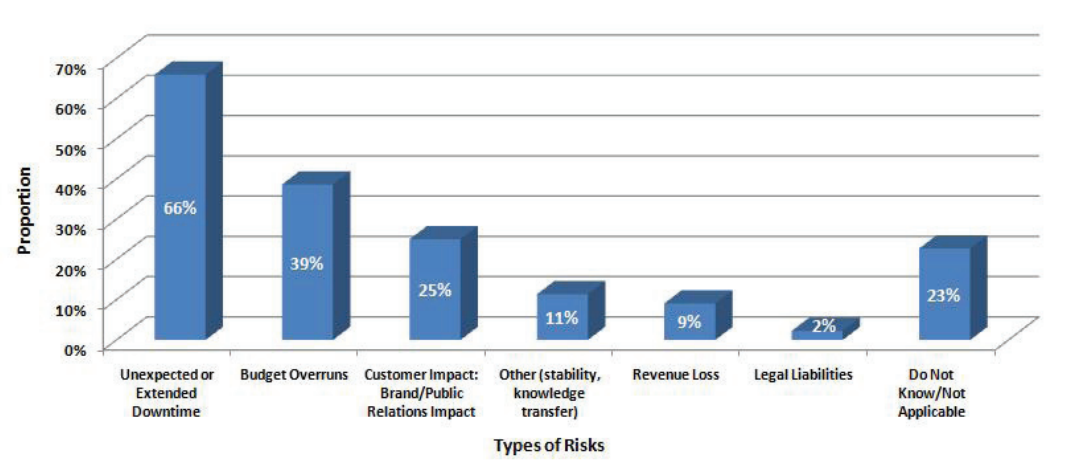
\includegraphics[width=13cm]{images/hitachi_survey}
  \caption{Hitachi survey on perceived risk in data migration \cite{paper:hitachi} }
  \label{fig:cpim-nosql}
\end{figure}

\newparagraph To mitigate those problems we want to extend the CPIM library to make it able to interact with \textit{Hegira} a migration system able to perform interoperable data migration and synchronization across column-based NoSQL databases \cite{paper:modaclouds-deliverable}. \textit{Hegira} is already able to migrate data offline, but in many cases this solution is not acceptable since this requires to turn off the application for a period of time that depends on the volume of data that needs to be migrated towards the new database. 
Downtime costs and risks of data loss can be problematic so, \textit{Hegira} was extended to be able to perform a live-migration of the data by keeping them synchronized on the source and the destination database.
This feature needs to be exploited at application level and thus we decided to embed it inside the CPIM NoSQL service, in order to make it as transparent as possible to the user.

\noindent The CPIM library needs to be aware of the state of both the synchronization and migration systems and acts accordingly intercepting user operation and sending data manipulation queries (DMQ) to the migration system which is in charge of keeping the data consistent across the replicated databases.

%--------------------------------------------------------------------------------
% Kundera extension
%--------------------------------------------------------------------------------
\chapter{Kundera extension}
\label{chap:kundera}
\section{Introduction}
In this chapter will be presented the way in which Kundera is supposed to be extended, the problems occurred in the process and how the community helped in achieving the result.
In section \ref{sec:kundera-datastore} are discussed the detail fo the extension for Google Datastore and in the section \ref{sec:kundera-table} the details for Azure Table.

\section{Kundera's Client Extension Framework}
Kundera as on open source project, thought that other developers could be interested in using it and extending its support to other datastore.
So in the wiki is presented the Client Extension Framework which provides a short description on how Kunders clients should work and provides the interfaces and classes that should be developed in order to make the client work properly.
\\
Looking at Kundera architecture, described in chapter \ref{chap:soa}, is clear the modularity on which Kundera has been developed. When dealing with classes JPA annotated, the Kundera core provides the necessary logic to fully support the JPA 2.1 specification and when it's time to interact with the underlying database (for persisting, updating or reading entities) it delegate the operation to the configured client in the persistence.xml file.
\\
The steps to build a new Kundera client, basically these are the blocks to be developed:
\begin{itemize}
\item the Client, which is the gateway to CRUD operations on database, except for queries;
\item the Client Factory, which is used by Kundera to instantiate the Client;
\item the Query implementor, which is used by Kundera to run JPA queries by invoking appropriate methods in Entity Readers;
\item the Entity Reader, which is used by Kundera to translate the queries into correct client
method calls;
\item optionally the Schema Manager, to support automatic schema generation.
\end{itemize}

\subsection{Approaching the extension}
It all seems quite simple but the problem is that the wiki is actually outdated. 
Two were the main problem in understaing what to do and how, firstly it turns out that the required interfaces are actualy a little different and also are the required methods
secondary, and slightly more time consuming, is that no hints are given on the structure and informations carried by the methods arguments.
The arguments carry data structures containing informations organized in the kundera metamodel which is the implementation of the JPA metamodel that contains all the information associated (throug annotations) to a class or a field.

Due to those problems and to shrink the developing time, the solution was to write on the Kundera google group page to ask the community for more updated infos about Kundera extension.
Briefly an answer has come and I've started a conversation with one of the developers of Kundera who helped me giving the updated infos for the Kundera's Client Extension Framework and tell me to look forward to the other client implementation for some examples. 
In light of the updated information it turns out that the Entity Reader was unnecessary and all the translation from JPA queries to datastore specific queries and their executions should be done in the Query Implementor.  

At this point since no answer were given about the Kundera metamodel, the most valid solution was to approach the extesion as a test driven development, so looking at the tests code of the other clients I've writed a set of unit tests one foreach feature (tests are analyzed in detail in chapter \ref{chap:eval}.
With the tests failing and the code of Kundera core was then possible to reverse engineer the arguments thath were not documented and thus be able to develop the new extensions.

\section{Google App Engine Datastore client}
\label{sec:kundera-datastore}
The first extension that has been done is the one for Google App Engine (GAE) Datastore the NoSQL solution available in the App Engine runtime, is a key-value storage build on top of Google BigTable.

\subsection{JPA identifier}
Google Datastore is a key-value storage in which the most basic unit that can be stored is an Entity which is identified by a Key and composed of Properties.
Entities Keys contains various information about the entity itself:
\begin{itemize}
\item the entity Kind, which is used to group entities of the same type;
\item an entity identifier, used to distinguish entities of the same type;
\item an optional parent entity. 
\end{itemize}
Inspired by the Google JPA implementation on Datastore the idea was to use the Java class representing the datastore Key as indentifier for the POJO but unfortunately this is not possible since Kundera support only a well known set of Java datatypes.

The adopted solution is to handle the key internally, each time an opertion is required on Datastore the key relative to the entity is builded, the key Kind is directly mapped to the table name and the Key identifier is the user defined id in the @Id annotation.

IDs can be specified by the user or automatically generated, there are three possibilities:
\begin{itemize}
\item @Id annotation on a String type field
\item @Id annotation on a Long type field
\item @Id annotation on a long type field
\end{itemize}
For each case the ID can be user specified before the persist operation but in case of ID auto-generated the field must be of type String and the generated ID will be a string representation of a random java UUID.

Auto-geenerated ID are supported by Kundera thorugh @GeneratedValue with AUTO or TABLE strategy, only AUTO strategy is supported as a random Java UUID. It was not possible to use the Datastore API to generate ids since is necessary to know the Kind of the entity to be persisted but neither the AUTO strategy nor the TABLE one provides this infomation at generation time.

\subsection{JPA relationships}
All the JPA supported relationships has been implemented in the client has been implemented like they would be in a RDBMS system.
So for One to One and One to Many relationships, where on the onwer side of the relationships there's a link to the non-owning side, the connection is keeped persisting within the entity the Key (Kind and identified) of the related entity.

For the Many to One relationships there would be to solutions:
\begin{itemize}
\item persist a list of Key of the related entities;
\item do not persist anything within the entity but fill the relationship with a query.
\end{itemize}
The second solution has been adopted since more consistent with the other client implementation and with the classic implementation of the relation type for RDBMS.

For the Many to Many relationships a join table is created based on the directives of the user specified in the annotations, then is filled each time one entity is persisted and is related with another one through a many to many relationship.

\subsection{Consistency}
In Datastore, entities are organized in Entity Groups based on their Ancestor Path, the ancestor path is a hierarchy containing the keys of the entities which are parents of the given one and thus are in the same entity group.

In Datastore consistency is managed through Entity Groups and so by defining the ancestor paths, entities within the same Entity Groups are managed in storng consistency, eventual consistency is used otherwise.

Datastore provide the possibility to create Ancestor path by defining them parent to other entities and is basically a task leaved to the user, no automated sorting or guessing is provided. Other wrapper around Datastore low-level API also leave this to the user, for example in Objectify the developer make use of an @Parent annotation that make the user able to specify the Ancestor Path.
Since JPA is well defined and adding such annotation will break the standard the only alternative way is trying to automatic guess the ancestor path.

Relationsips are clearly a good indicator when trying to guess if two entitiy kind can be hirearchically related:
\begin{itemize}
\item One to Many, since ther's a "many" side which is the non-owning side of the relationship the owning side can be clear used as parent for every entity in the "many" side;
\item Many to One, this is the inverse of the previous type and thus entities sould be already organized;
\item One to One, can be treated like the One to Many
\item Many to Many, in this case since there's a join table between the entities there are several solutions:
\begin{itemize}
\item put the join table and the non-owning entities parent to the owning ones;
\item put all the join table, the entities on the owning side and the ones on the non-owning side under a common fictitious root entity kind
\end{itemize}
\end{itemize}

This unfourtanently is not conventien since there's lot of possibilities, thinks for the Many to Many case but more important is that if an entity is in more than one on those relationships is not possible to prioritize them and choose unless asking to the user which is the case, furthermore when declaring a entity parent to another is always necessary to know the Key of the parent beside the Key of the entity itself to be able to retrieve it from Datastore and as Kundera is structured this kind of information is not available in the client but must be serached inside the kundera metadata when possible.

For those reasons was not possible without causing strange behaviours, automatically guess the Ancestor Paths through JPA relationships so at the end is not possible for the user to manage entity consistency, each entity is stored in a separated entity group identified by its Kind (the name of the JPA table associated to the entity).

\subsection{Other JPA features}

\subsubsection{Embedded entities}

\subsubsection{Collection fields}

\subsubsection{Enumeration fields}

\subsection{Queries}

\subsection{Schema Manager}
Schema manager as required by Kundera has to exploit four cases:
\begin{itemize}
\item validate which validates schema tables based on entity definition.
\item update which updates schema tables based on entity definition.
\item create which schema tables based on entity definitions.
\item create\textunderscore drop which drops (if exists) schema, then creates schema tables based on entity definitions.
\end{itemize}
The first two cases are quite useless for a Datastore since ther'se no fixed schema for entities, entities with same Kind can have different Properties withouth restriction.
Also the "create" case is usless for Datastore since if a new entity of an unknown Kind is persisted it's created withoud the need to explicitly define it first as a "table".
The remanining case "create\textunderscore drop" will so just drop the current schema deleting all the entities af all the Kinds without recreating schema since it construct by itself.

\section{Azure Table client}
\label{sec:kundera-table}
Table is the NoSQL solution developed by Microsoft, is a key-value storage and it's available inside Azure environment.

\subsection{JPA identifier}

\subsection{JPA relationships}
Also for Azure Table, to keep uniform the extension behaviour, all the JPA supported relationships has been implemented in the client has been implemented like they would be in a RDBMS system.

The only difference is that when is needed to keep a reference to another entity in the owning side of a relationship is persisted within the entity the partition key and the row key of the related entity since the pair partition key and row key universally identify an entity.

\subsection{Consistency}
In Azure Table strong consistency is guaranteed while entities are stored within the same partition key otherwise consistency will be eventual. IDs are supported only in field of type String (so only a String field can be annotated with @Id). User can define IDs both with or without partition key.

\subsubsection{Define both row key and partition key}
This can be done in two ways:
\begin{itemize}
\item using AzureTableKey.asString method by passing both partition key and row key to obtain a string representation of the whole key and assign it to the entity ID field before persist.
\item manually define the entity ID before persist the entity, the string must follow the pattern partitionKey\textunderscore rowKey.
\end{itemize}

\subsubsection{Define only the row key}
If only the row key is defined, the partition key is implicitly the default one (which can be set in a datastore specific properties file).

There are three ways to do this:
\begin{itemize}
\item auto-generated IDs (the row key is a random java UUID)
\item manually define the entity ID before persist the entity
\item using AzureTableKey.asString passing as parameter the desired row key and assign its result to the entity ID field before persist.
\end{itemize}

\subsection{Other JPA features}

\subsubsection{Embedded entities}

\subsubsection{Collection fields}

\subsubsection{Enumeration fields}

\subsection{Queries}

\subsection{Schema Manager}
Schema manager as required by Kundera has to exploit four cases:
\begin{itemize}
\item validate which validates schema tables based on entity definition.
\item update which updates schema tables based on entity definition.
\item create which schema tables based on entity definitions.
\item create\textunderscore drop which drops (if exists) schema, then creates schema tables based on entity definitions.
\end{itemize}
Here, like Google Datastore, the first two cases are quite useless for Azure Table since ther'se no fixed schema and entities within the same Table can have different properties withouth restriction.

Azure Table need that the Table in which entities are stored exists before trying to create entities so the "create" case simply iterate over all table names and creates it in the database. 
For the "create\textunderscore drop" case, all tables are dropped (and so all the contained entities) and re-created.

\section{Summary}
In this chpater has been introduced in details how Kundera extension should been developed, the problem encountered during the development, how tey've been addressed and the detail of the implementation of the two extensions including what the feature currently supported.
In the next chapter will be explained how has been possible to integrate Kundera into CPIM as part of the NoSQL service.


%--------------------------------------------------------------------------------
% CPIM extension
%--------------------------------------------------------------------------------
\chapter{CPIM extension}
\label{chap:cpim}
\section{Introduction}
This chapter presents the CPIM library extension. Sections \ref{sec:cpim-architecture} and \ref{sec:kundera-integration} describe the previous state of the NoSQL service in the CPIM and the changes made to integrate Kundera as unique persistence provider and the problems faced during the process.

\noindent From section \ref{sec:hegira} up to section \ref{sec:data-interoperability} describe the various parts we developed to support \textit{Hegira}, an interoperable data migration sand synchronization system for NoSQL databases \cite{paper:modaclouds-deliverable}, the supported features and the design choices that have been put in place. 

\section{CPIM architecture}
\label{sec:cpim-architecture}
In order to be able to expose a common interface for the multiple services supported by the library, CPIM adopts heavily the factory and singleton patterns.

\noindent The main access point of the library is the \texttt{MF} (Manager Factory) a singleton object which is responsible of reading the configuration files and exposing a set of methods that will build instances for the service factories.
The initialization is done through a first call to \texttt{MF.getFactory()} method which reads the configuration files and build an instance of the \texttt{CloudMetadata} class. 

\noindent This class will be referenced by all the other services and it contains all the information stored in the configuration files.
 
\newparagraph The CPIM library is organized in several packages, each of which is responsible of a particular service.
\noindent Each service exposes a factory class which is invoked through the \texttt{MF} factory; the service factory maintains a singleton instance of the provider-specific service implementation which is built, at the first call, based on the configuration available inside the singleton instance of \texttt{CloudMetadata}.
The result of this process is that with the same method call, based on the configuration file, can be instantiated different service implementation.

\subsection{NoSQL service}
The architecture of the NoSQL service before this work has been reported in figure \ref{fig:cpim-nosql}.

\begin{figure}[tbh]
  \centering
  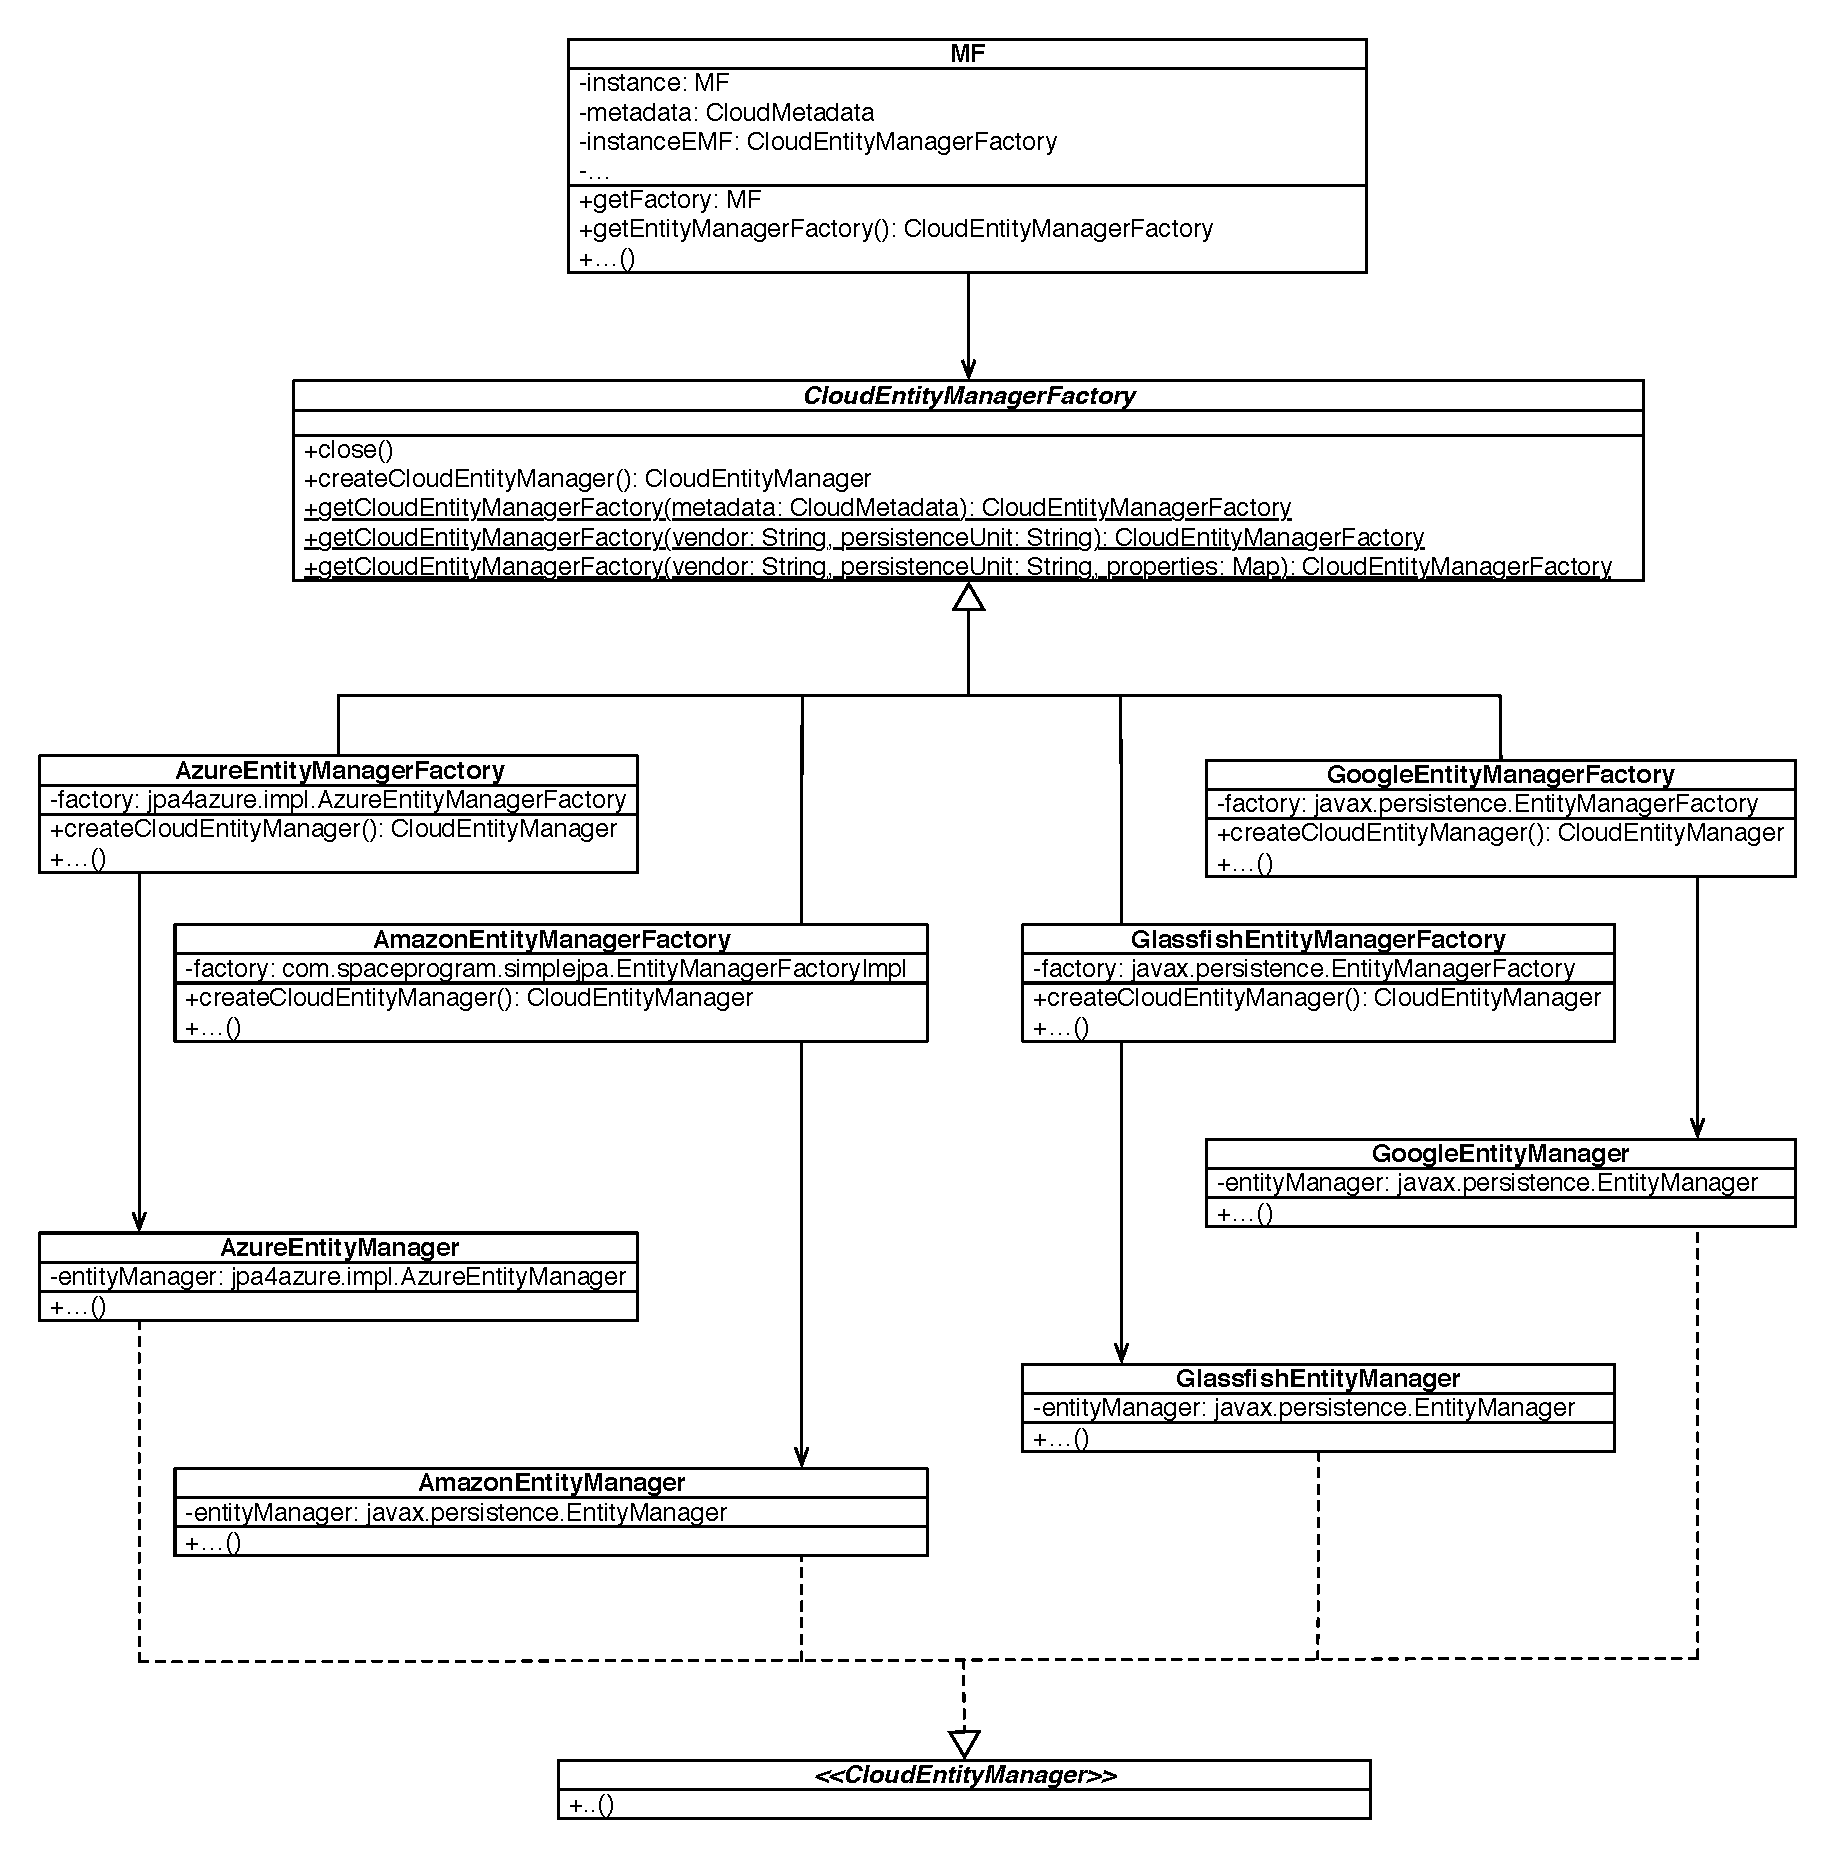
\includegraphics[width=14cm]{images/cpim_nosql_old}
  \caption{NoSQL service architecture}
  \label{fig:cpim-nosql}
\end{figure}

\noindent To use the service, the first step is to instantiate a \texttt{CloudEntityManagerFactory} and, depending on the configuration file, this factory instantiates the vendor specific factory. For example, in case Google is chosen as vendor, the instantiated factory will be \texttt{GoogleEntityManagerFactory}. 
Each provider-specific \texttt{EntityManagerFactory} is responsible of instantiating an \texttt{EntityManager} which is the gateway to the underlying database. All vendor-specific \texttt{EntityManager}(s) implement the common \texttt{CloudEntityManager} interface to achieve uniformity in methods and behavior.
The various implementation of the \texttt{CloudEntityManager} delegates every method call to the vendor-specific persistence provider. 

\newparagraph The JPA is not a default language for NoSQL but, due to its wide usage among Java developers, several JPA implementations have been built for various NoSQL databases (both developed by the vendor of the NoSQL storage or by the community).
This means that to support the NoSQL service through the JPA interface, an implementation of the JPA interface must be found or developed \textit{ad hoc}. For this reason there were three different persistence providers in the CPIM library, one for each cloud provider:
\begin{itemize}
\item for \textit{Google Datastore} an official JPA implementation (available inside the SDK) was used;
\item for \textit{Amazon SimpleDB} it used \textbf{SimpleJPA}, a third-party implementation of the JPA interface;
\item for \textit{Azure Tables} it used \textbf{jpa4azure}, a third-party implementation of the JPA interface.
\end{itemize}

\noindent There are a couple of things to notice: Amazon SimpleDB has been deprecated in favor of DynamoDB and \textit{jpa4azure} is not being maintained anymore, therefore the CPIM library needs to be updated in order to get rid of those outdated software.

\section{Kundera integration}
\label{sec:kundera-integration}
To solve these problems and reduce the number of software on which the CPIM relies to provide the NoSQL service, the proposed solution is to modify the current CPIM architecture with a unique persistence provider that has been identified in Kundera.

\newparagraph The renewed architecture is resumed in figure \ref{fig:cpim-kundera} in which the benefit of having a single JPA provider are clearly visible, the architecture is slightly less articulated and no check on the selected underlying technology is needed since this is handled by Kundera, while reading the \textit{persistence.xml} file, in which the user defines the datastores he is interested in.
Another benefit of this architecture is that the choice of the NoSQL technology is not bound to the vendor specified in the CPIM configuration file anymore, in fact, it is possible, by configuring the \textit{persistence.xml}, to deploy the application in one of the supported PaaS providers and choose to persist the data in a NoSQL database of another provider. Moreover it is possible to exploit the Kundera polyglot persistency to persist part of the data in a database and another part in another one, defining the persistence units accordingly.

\begin{figure}[tbh]
  \centering
  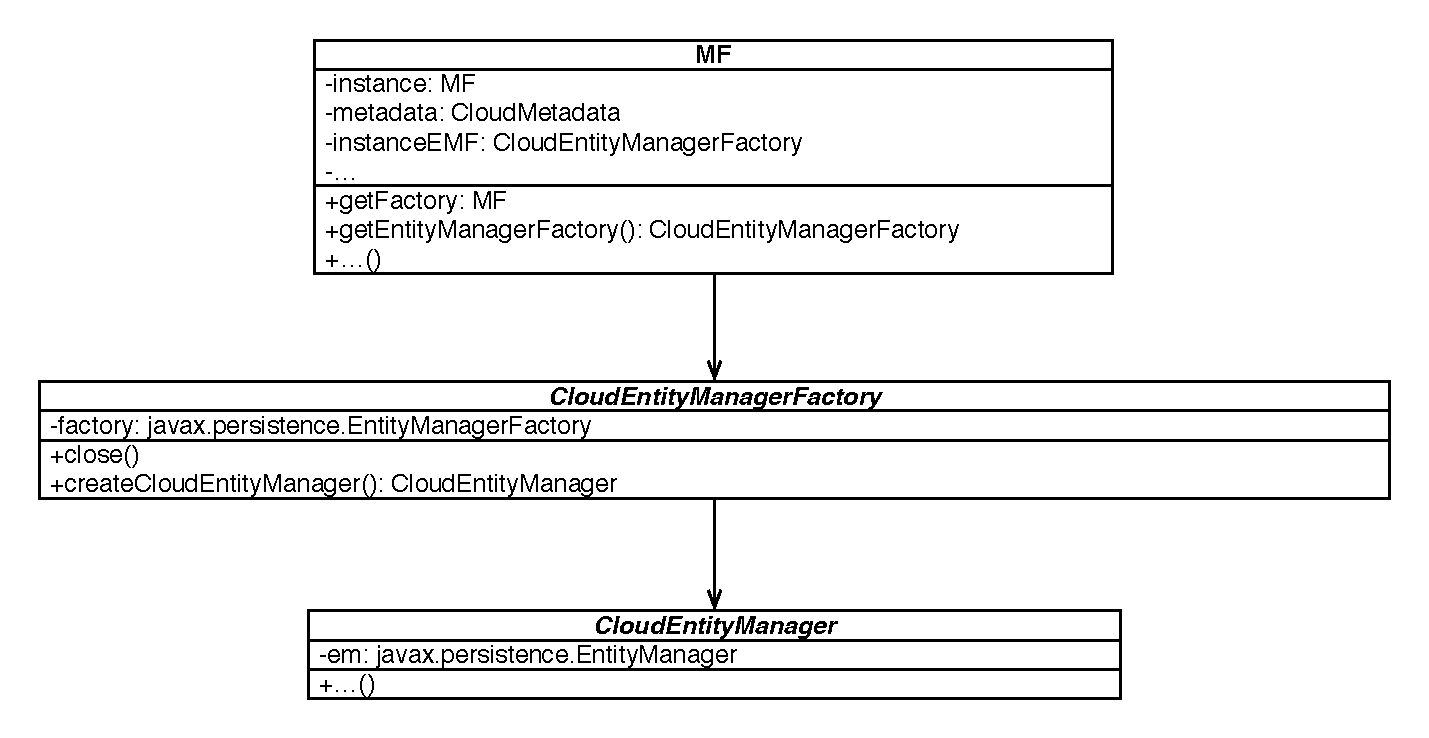
\includegraphics[width=14cm]{images/cpim_nosql_kundera}
  \caption{The modified NoSQL service architecture}
  \label{fig:cpim-kundera}
\end{figure}

\noindent The actual implementation is completely provider agnostic in the sense that actually Kundera is not required as dependency and in fact it is not listed as a dependency for the CPIM. At run-time, when a Kundera client will be listed among the dependencies of the user application, as well as the CPIM library, the persistence provider dependency will be satisfied.

\noindent This provider agnostic implementation is due to the fact that the \texttt{CloudEntityManagerFactory} and the \texttt{CloudEntityManager} respectively implement the JPA interfaces \texttt{EntityManagerFactory}  and \texttt{EntityManager}.
The actual call to the run-time provider is made within the \texttt{CloudEntityManager} that, on construction, instantiate an instances of the provider \texttt{EntityManager} and uses that reference to delegate every method execution to it.

\noindent This can seem an over-designed architecture, but it turns out to be extremely necessary in order to provide a transparent interaction with the migration system, as it will explained later on in this chapter.

\subsection{Problems encountered}
Kundera provides an uniform access through the JPA interface, independently from the NoSQL provider which is being used. The desired database is defined in the \textit{persistence.xml} file through the \texttt{kundera.client.lookup.class} property. For this reason all the old libraries that provide a JPA implementation for a specific vendor can be removed from the CPIM. 
This tentative of cleaning the dependency of the CPIM caused two main problems:
\begin{enumerate}
\item \textit{jpa4azure} turns out to be used also for Queue and Blob service of Windows Azure;
\item Kundera seems to have problems when multiple persistence providers are found in the classpath and currently no way to force the selection of Kundera as persistence provider has been found(besides specifying it in the \textit{persistence.xml} file).
\end{enumerate} 

\noindent To solve the first problem, the code of the extended version of \textit{jpa4azure} has been inspected. We found that the library was previously extended to support some missing functionalities of the JPA interface and contained two main packages:
\begin{itemize}
\item \texttt{jpa4azure}, which contained the code that implements the JPA interface;
\item \texttt{com.windowsazure.samples}, which contains the code to ease the communication with the Azure services.
\end{itemize}
The \texttt{jpa4azure} package has been removed and the library rebuilt since the other package is the one used in the Blob and Queue service. Its possible to completely remove \texttt{jpa4azure} but is necessary to rewrite also the CPIM Blob storage service for Azure using the API provided by the Azure SDK.

\newparagraph Removing the \texttt{jpa4azure} library caused unexpected errors in CPIM in the code of the Queue service. After some investigations, turns out that, when \textit{jpa4azure} was extended, the class \texttt{AzureQueueManagerFactory} were introduced.
The problem was that \texttt{AzureQueueManagerFactory} make use of the JPA interface to communicate with the Queue service of Azure and thus by removing the support to the JPA interface we have lost the support for Azure Queue service.
A solution to this would be to rewrite the CPIM Queue service for Azure, using the API provided by the Azure SDK.

\section{Hegira integration}
\label{sec:hegira}
To support data synchronization and migration, the NoSQL service was further modified to integrate \textbf{Hegira} \cite{thesis:marco}. An high level schema of the interaction we want to achieve is reported in figure \ref{fig:high-level-interaction}

\begin{figure}[tbh]
  \centering
  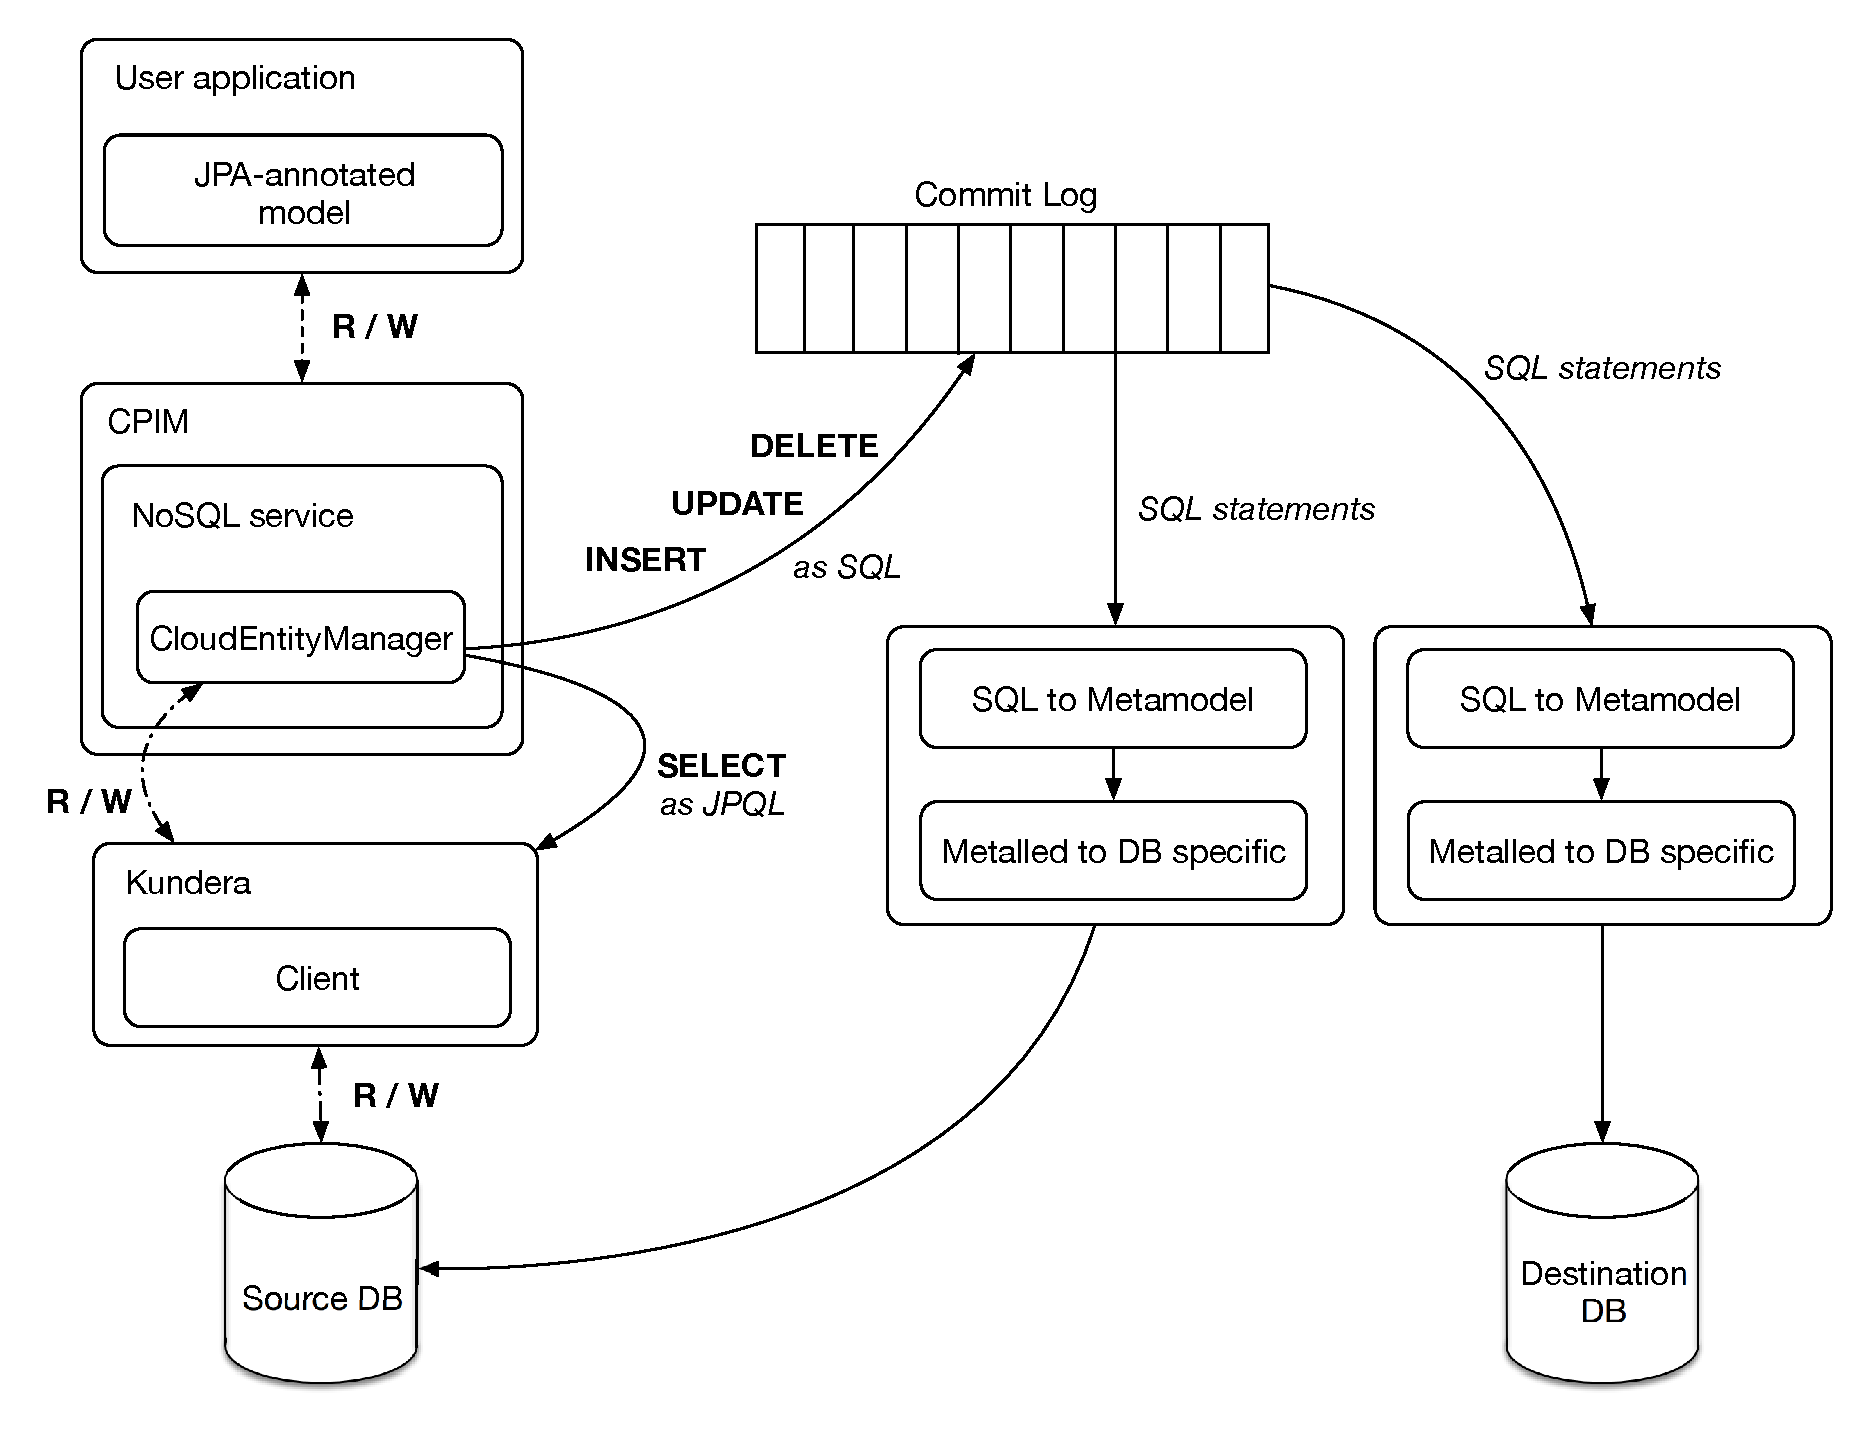
\includegraphics[width=12cm]{images/high_level_interaction}
  \caption{High level schema of interaction}
  \label{fig:high-level-interaction}
\end{figure} 

\noindent In the above schema, \textit{dashed} lines represents the normal flow of data from the user application to the local database, the filled ones represents the behavior in case a migration is in process.

\noindent The CPIM library needs to connect to the migration system in order to understand when a migration is in progress and in that case only bypass the interaction with Kundera (for data manipulation operations) by building a string representation of the user query as a SQL statement. Once this SQL generated string is sent to the \textit{Hegira} commit log that pop the statements and translate them into a datastore-specific operation.

\subsection{Migration Manager}
Interaction with the migration system is handled primarily by the \texttt{MigrationManager} class which follows a state pattern represented in the class diagram \ref{fig:migration-class-diagram}. 
 
\begin{figure}[tbh]
  \centering
  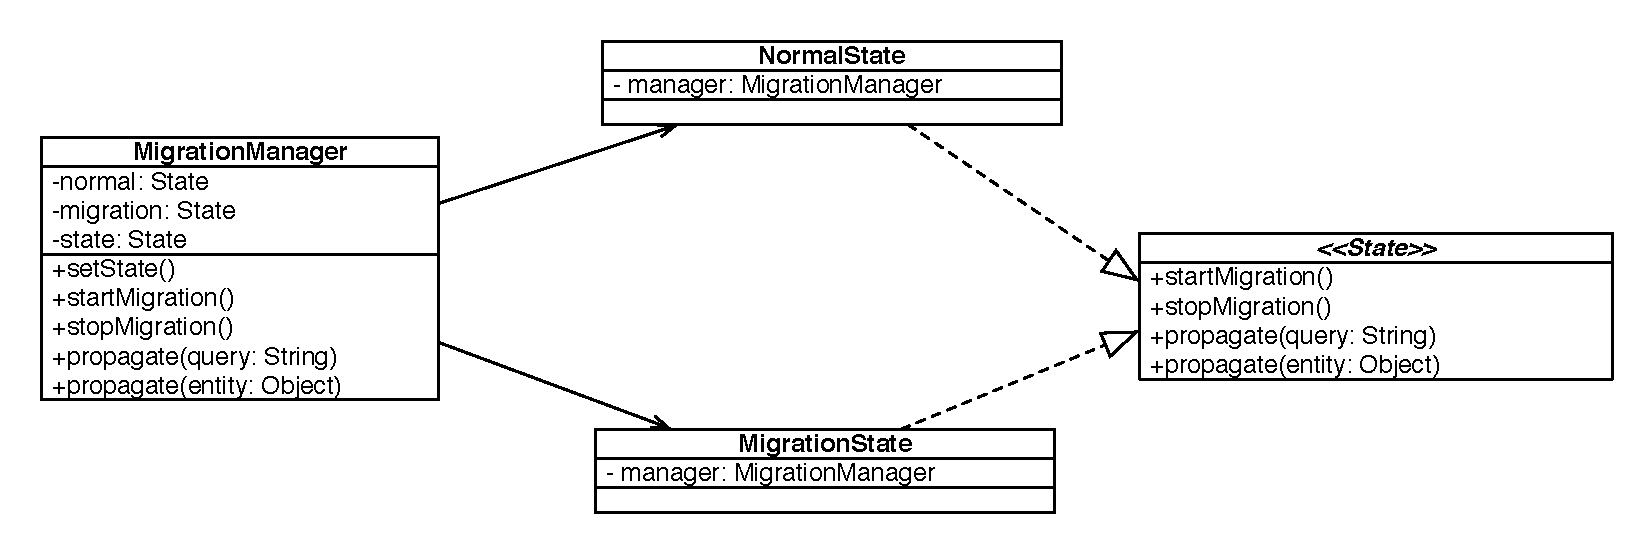
\includegraphics[width=14cm]{images/migration_class_diagram}
  \caption{\texttt{MigrationManager} class diagram}
  \label{fig:migration-class-diagram}
\end{figure} 

\noindent The pattern allows to the \texttt{MigrationManager} to delegate the method execution to the current state, the state diagram is the one represented in figure \ref{fig:migration-fsa} and is composed by two states \texttt{Migration} and \texttt{Normal} that encapsulate the required behavior.
    
\begin{figure}[tbh]
  \centering
  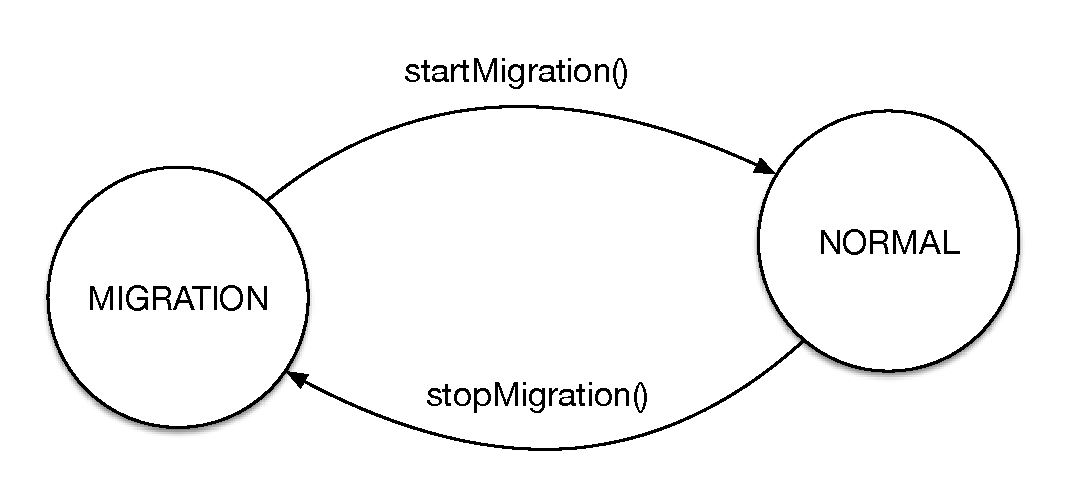
\includegraphics[width=6cm]{images/migration_fsa}
  \caption{\texttt{MigrationManager} states}
  \label{fig:migration-fsa}
\end{figure} 

\section{Intercept user operations}
The first operation that needs to be analyzed is whether it is possible to intercept user operations in a way that is completely transparent to the user.
The operations that we want to intercept are the insert, update and delete operations, in that, they are the operations that alter data and, thus, are the ones that the synchronization system needs to process.

\subsection{Intercepting CRUD operations}
CRUD operations are handled by the \texttt{EntityManager}, three are the methods that need to be intercepted:
\begin{itemize}
\item \texttt{EntityManager.persist(Object entity)} for insert operations;
\item \texttt{EntityManager.merge(Object entity)} for update operations;
\item \texttt{EntityManager.remove(Object entity)} for delete operations.
\end{itemize}
\noindent The user does not invoke methods directly on the provider entity manager, but he interacts with the persistence provider, through the \texttt{CloudEntityManager} class. In the standard implementation (i.e. without the support for the migration system) the \texttt{CloudEntityManager}, delegates every method call to the provider entity manager; hence, in order to integrate the  migration and synchronization logic, the methods mentioned above should contain the application of logic shown in the snippet of code \ref{code:isMigrating}, which takes as an taking as example, the update operation.

\begin{lstlisting}[language=Java, caption=Integrate migration logic, label=code:isMigrating]
public <T> T merge(T entity) {
    if (MigrationManager.isMigrating()) {
        MigrationManager.propagate(entity, OperationType.UPDATE);
        return entity;
    } else {
        return delegate.merge(entity);
    }
}
\end{lstlisting}

\noindent In case of data migration, the provider is bypassed and a call to the \texttt{propagate} method is visible. The call accepts two arguments: the entity to be converted to a SQL statement and the operation that needs to be generated. The method is called on the \texttt{MigrationManager} which then delegates the execution to the current state (which should be the migration one). The migration state \texttt{propagate} method is responsible for building the requested statements, using the statement builders and then sending the generated statements to \textit{Hegira} commit log. Both actions are described in detail in the following sections.

\subsection{Intercepting queries}
Looking at the JPQL specification \cite{book:projpa2} it turns out that JPQL does not support \textit{INSERT} statements and so the only way a user has to persist some entities is by means of \texttt{EntityManager.persist(Object entity)} method, which was described in the previous section; so, only the remaining queries (\textit{UPDATE} and \textit{DELETE}) need to be intercepted as query.

\noindent The JPA interface provides several ways to build and execute queries, all available by calling the proper methods defined in the \texttt{EntityManager} interface: 
\begin{itemize}
\item \texttt{createQuery}, which creates a \texttt{Query} instance from JPQL query string;
\item \texttt{createQuery}, which creates a \texttt{Query} instance from an instance of \texttt{CriteriaQuery};
\item \texttt{createNamedQuery}, which creates a \texttt{Query} instance from a JPQL query identified by name and declared statically on classes; 
\item \texttt{createNativeQuery}, which creates a \texttt{Query} instance from a string representation of the underlying database specific SQL dialect.
\end{itemize}
 
\noindent Native queries are not supported by Kundera, moreover the migration system tries to abstract from the specific database query language, hence there is no point in supporting this kind of queries. \texttt{createQuery} and \texttt{createNamedQuery} are supported, instead query creation through \texttt{CriteriaQuery} is currently not supported.

\newparagraph The JPA does not provide, through the \texttt{Query} interface, a way to get the JPQL representation of the query. Queries are supposed to be written as method argument when creating them through the \texttt{EntityManager} or called by name if they are defined as named queries upon some class.
This was actually a problem since, in order to be able to parse the query, its JPQL representation is crucial.

\noindent The easiest solution was to implement the interfaces for \texttt{Query} and \texttt{TypedQuery} respectively with the classes \texttt{CloudQuery} and \texttt{TypedCloudQuery}. 

\noindent The wrapping of the persistence provider queries is achieved in the entity manager and it is performed by the query creation method both for the \texttt{Query} and \texttt{TypedQuery} returned objects. The actual JPA query generation is delegated to the persistence provider; before returning to the user, the result query is wrapped in a \texttt{CloudQuery} that contains both the generated query and its string representation.

\newparagraph For named queries things are little trickier since the user create instance of \texttt{Query} or \texttt{TypedQuery} just by passing the query name.
\noindent As can be seen from the code snippet \ref{code:wrap-named-queries}, named queries meta-data are maintained inside the \texttt{PersistenceMetadata} class. This class, besides maintaining information about named queries, principally maintains a mapping between table names and their class canonical name (full package plus the class name). The first time this class is queried, its content is created (since it is a singleton instance) and it does not directly read the  configuration files, but the \texttt{CloudMetadata} instance that has been modified to include all the required parameters that needs to be read from configuration files. 
The information of table to class mapping is required for statements building and for sequence number handling both described in the following sections.

\begin{lstlisting}[language=Java, caption=Wrap named queries, label=code:wrap-named-queries]
public Query createNamedQuery(String name) {
    String queryString = PersistenceMetadata.getNamedQuery(name);
    Query queryInstance = delegate.createNamedQuery(name)
    return new CloudQuery(queryString, queryInstance);
}
\end{lstlisting}

\section{Adding support for data synchronization}
\label{sec:sync}
In this section we report the solution adopted for supporting \textit{Hegira} data synchronization \cite{paper:modaclouds-deliverable}, which allows to perform online data migration.

\noindent A special look needs to be reserved to the insert operation. When the user updates or delete an entity no matter if through the entity manager or through a query, he already knows the that entity identifier, since the insert operation has already persisted that entity into the underlying database and thus generated on identifier.
Since we want to support the migration system, the user cannot define its own identifiers, but they need to be assigned from the migration system itself.
The main caveats is that such assignment needs to be made even if the migration is not running yet so the identifier assignment has to be made in two cases:
\begin{enumerate}
\item insert statements built from persist operation during a migration phase
\item \textit{standard} insert operation through the entity manager during a normal state
\end{enumerate}

\noindent The solution is actually quite simple since everything can be checked inside the \texttt{EntityManager.persist} method as described in the snippet of code \ref{code:persist}.

\begin{lstlisting}[language=Java, caption=Persist operation, label=code:persist]
public void persist(Object entity) {
    if (MigrationManager.isMigrating()) {
        MigrationManager.propagate(entity, OperationType.INSERT);
    } else {
        String tableName = ReflectionUtils.getJPATableName(entity);
        int id = SeqNumberProvider.getNextSequenceNumber(tableName);
        ReflectionUtils.setEntityId(entity, id);
        delegate.persist(entity);
    }
}
\end{lstlisting}

\noindent In the code snippet is visible a call to the  \texttt{SeqNumberProvider} class, which is the class responsible of actually interacting with the Hegira component gabdling and handle the \textit{sequence numbers} generation i.e., the entities identifiers defined by Hegira to achieve fault-tolerant data migration and synchronization. 

\subsubsection{Handling the sequence numbers}
The sequence numbers are handled by the class \texttt{SeqNumberProvider}, a singleton instance that provides a simple way to get the assigned sequence numbers per table.
\noindent The class diagram of this component and of the component it interacts with is shown in figure \ref{fig:seq-provider}

\begin{figure}[tbh]
  \centering
  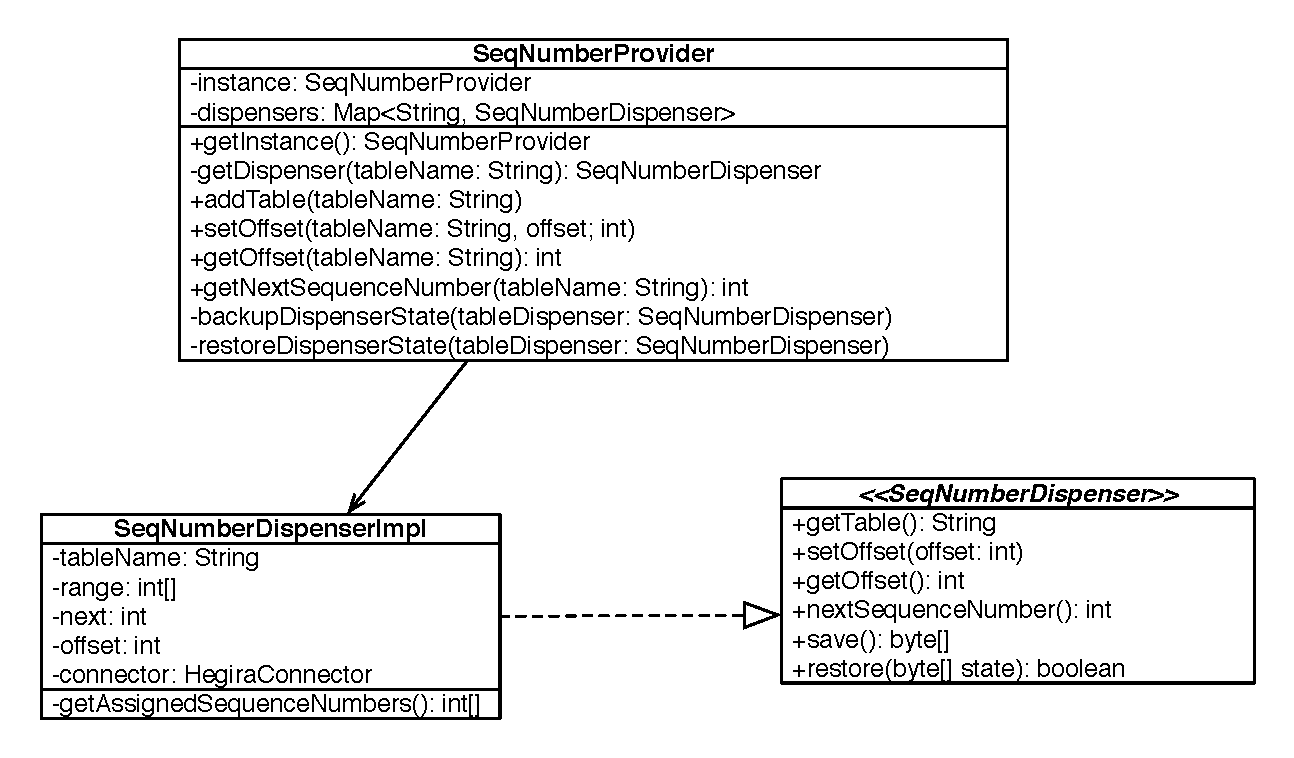
\includegraphics[width=12cm]{images/seq_provider}
  \caption{Sequence numbers handling architecture}
  \label{fig:seq-provider}
\end{figure} 

\noindent The \texttt{SeqNumberProvider} keeps an instance of \texttt{SeqNumberDispenser} for each table that needs to be persisted, and it is responsible of:
\begin{enumerate}
\item providing a unique access point when requesting the next assigned sequence number for a table;
\item initializing or restoring the state of the dispenser for each table.
\end{enumerate}
\noindent The first point is performed through the method \texttt{getNextSequenceNumber(String tableName)} that delegates the operation to the correct \texttt{SeqNumberDispenser} associated to the requested table.
Since \texttt{SeqNumberDispenser} is an interface, the actual implementation is delegated to the \texttt{SeqNumberDispenserImpl} class, this mechanism has been used to be able to create more dispensers with different logic.
\noindent The \texttt{SeqNumberDispenserImpl} class maintains internally the assigned range of identifiers provided by the synchronization system by specifying the first and the last element of the range. The class consumes, one by one, the identifiers in the range and when the range has been completed requests the next range. This mechanism is internally handled, in fact the \texttt{SeqNumberProvider} is only required to call the \texttt{getNextSequenceNumber()} method on the dispenser.

\noindent The size of the range of sequence numbers requested to the synchronization system, that is used by the \texttt{SeqNumberDispenser}, has been made configurable at run-time. A default range size can be set using the \textit{migration.xml} file, otherwise, a call to the \texttt{setOffset(String tableName, int offset)} method on the \texttt{SeqNumberProvider}, will change, at-runtime, the size of the range of the \texttt{SeqNumberDispenser} responsible for the specified table.

\newparagraph The second functionality is achieved by requesting the state representation to the \texttt{SeqNumberDispenser}(s) (as a \texttt{byte} array), calling the method \texttt{save()} on the dispensers and, then, saving it to a Blob storage or to a file depending on the configuration specified inside the \textit{migration.xml} file, described in Appendix \ref{app:migration}. 
\noindent The restoring phase is performed just after construction, if a backup exists either on file or on the Blob storage, the method \texttt{restore(byte[] state)} is called on the dispensers giving them its state representation to restore.
In this mechanism, the \texttt{SeqNumberProvider} is completely agnostic with respect to the actual state representation chosen by the \texttt{SeqNumberDispenser}(s). This makes future extensibility more easy and less constrained.

\noindent The list of all the tables to be persisted is retrieved from the \texttt{PersistenceMetadata} previously mentioned for named queries.
 
\subsection{Contacting the synchronization system}
The interaction with the synchronization system as now was only described as a method call. Those calls are made on an external library (\texttt{zkWrapper}) which provides an interface to a zookeeper instance, in order to communicate with the synchronization system, and to receive the assigned sequence numbers.
Since the zookeeper library uses threads to handle communication, it was not possible to use this library for Google App Engine since the App Engine run-time does not permit to spawn thread.
The main reasons to communicate with the synchronization system are:
\begin{itemize}
\item the migration state listener modifies the \texttt{MigrationManager} state accordingly;
\item the \texttt{SeqNumberDispenser} that needs to retrieve the sequence number assigned to tables.
\end{itemize} 
\noindent The adopted solution was to modify the \texttt{zkWrapper} library to include an HTTP version that handles the calls not by connecting directly to a zookeeper instance, but contacting a remote server through some defined API that ultimately interacts with the migration system.

\newparagraph A simple structure has been built to make both the \texttt{MigrationManager} and the \texttt{SeqNumberDispenser}(s) transparent to the type of client that is used to retrieve information from the synchronization system. The architecture is shown in figure \ref{fig:zk-adapter}

\begin{figure}[tbh]
  \centering
  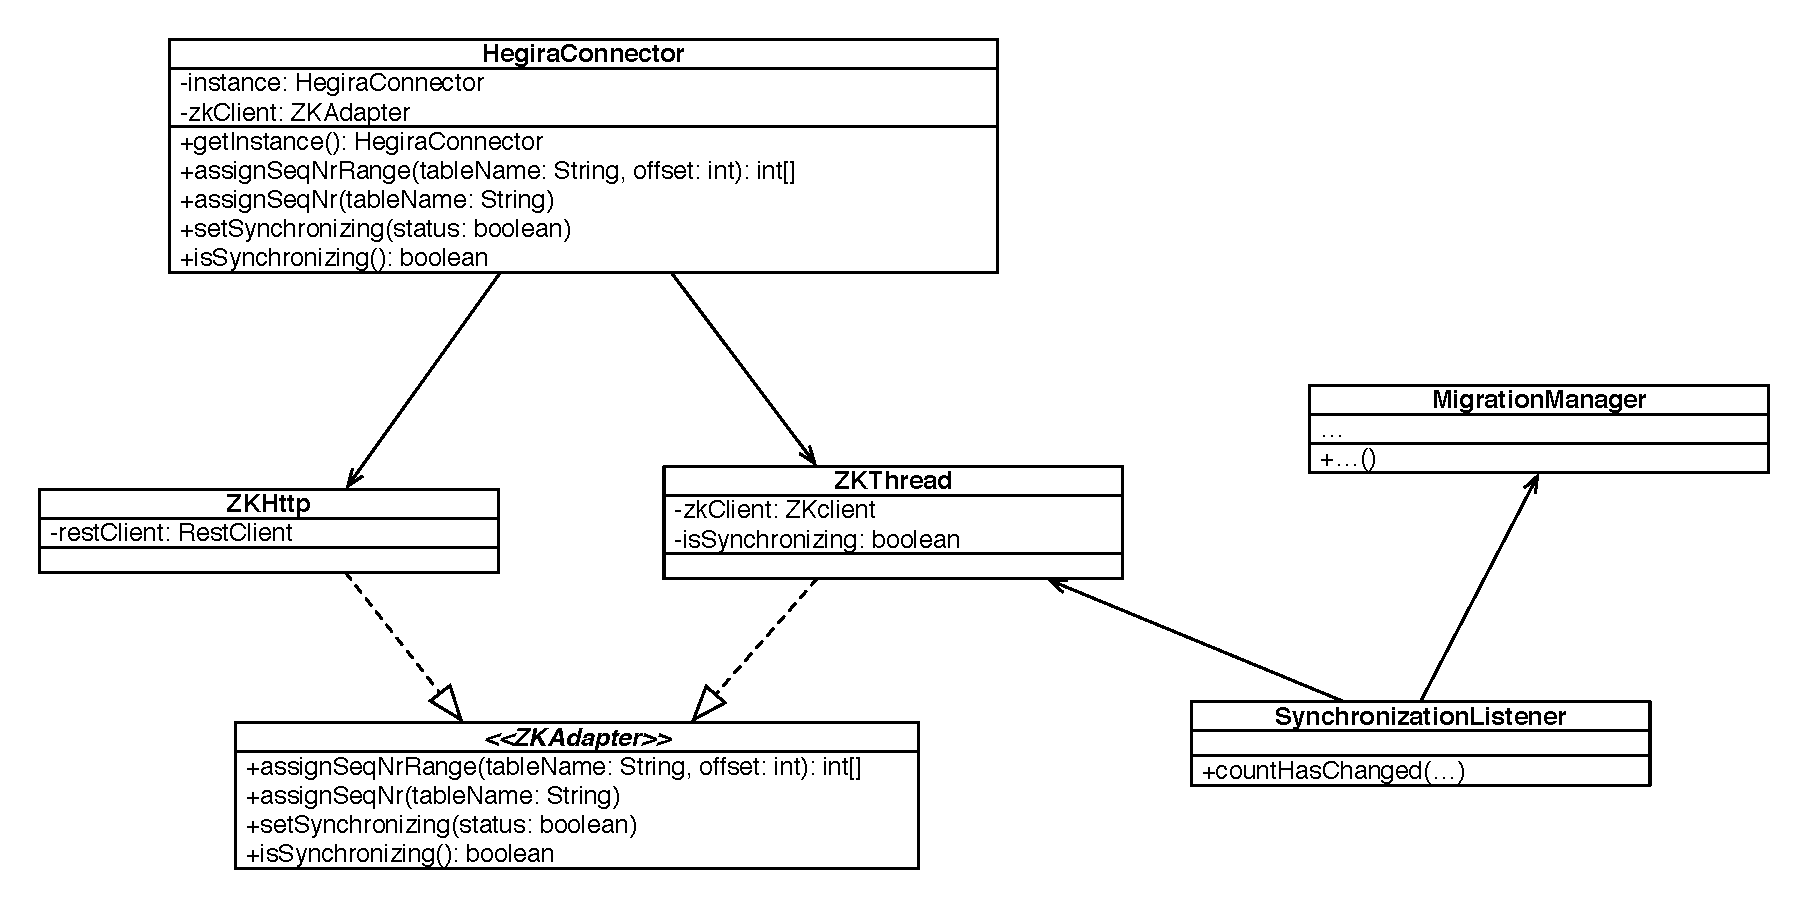
\includegraphics[width=14cm]{images/zk_adapter}
  \caption{Contacting the synchronization system}
  \label{fig:zk-adapter}
\end{figure} 

\noindent The \texttt{HegiraConnector} is the class responsible of deciding which kind of client needs to be instantiated, the decision is done by reading the configuration that the user specified in the \textit{migration.xml} file, which is parsed by the CPIM and kept in the \texttt{CloudMetadata} class. The \texttt{HegiraConnector}  keeps internally an instance of the chosen client and provides access to its method by delegation.
The two available clients implements the interface \texttt{ZKAdapter}, built to uniform the methods of the two implementations.

\paragraph{Thread-based client} If the user deploies the application on a thread-capable client, and configures the \textit{migration.xml} accordingly, an instance of \texttt{ZKThread} is built. This version of the client directly uses the implementation of the library \texttt{zkWrapper} (since there should not be any problem in thread spawning).
The \texttt{isSynchronizing()} method returns a value which is kept inside the \texttt{ZKThread} instance and is queried by the \texttt{MigrationManager}.
Both the state of the \texttt{MigrationManager} and the value inside \texttt{ZKThread} are modified by the \texttt{SynchronizationListener} which is asynchronously notified by the \texttt{zkWrapper} library when the synchronization state changes.

\paragraph{HTTP-based client} In the case in which threads are not supported by the cloud provider (for example on PaaS), the client version that is instantiated (by looking at the configuration) is \texttt{ZKHttp} which uses the API-caller added to the \texttt{zkWrapper} library.
Since no listener can be register to be asynchronously notified of a change in the synchronization state, each call of the \texttt{MigrationManager} to the method \texttt{isSynchronizing()} will perform an API call to the remote server, which will return the state of the synchronization system.

\newparagraph Before focusing on the statements building, it may be useful to visualize the interaction so far presented in the high-level flow chart presented in figure \ref{fig:flow-chart}.

\begin{figure}[tbh]
  \centering
  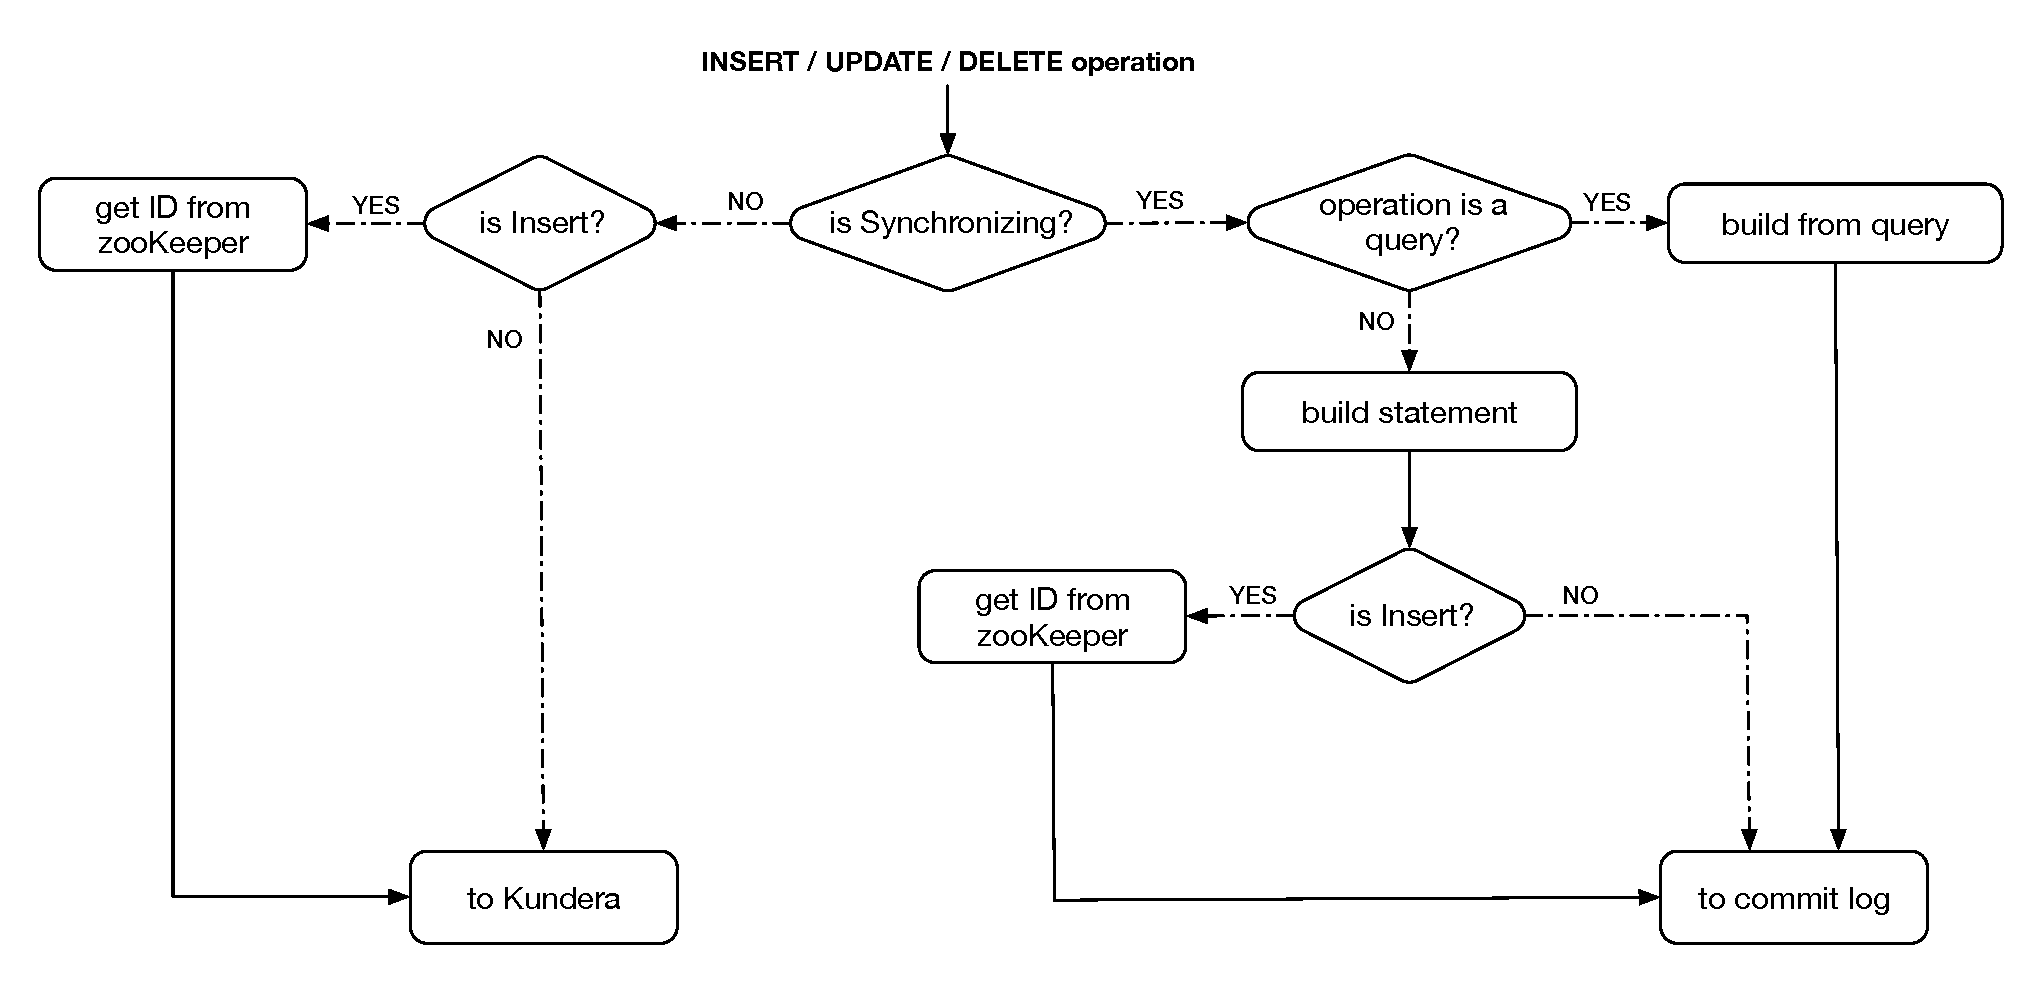
\includegraphics[width=13.5cm]{images/flow_chart}
  \caption{Interaction flow chart}
  \label{fig:flow-chart}
\end{figure} 

\section{Build statements from user operations}
\label{sec:statements}
In the previous section we have focused on the sequence number retrieval, in this section we will focus on the generation of the Data manipulation queries (DMQs) to be sent to \textit{Hegira} commit-log.

\newparagraph In order to be able to create SQL-like statements both from queries and from objects, the first step has been to introduce the \textit{statement} concept in the CPIM library. This has been done through the abstract class \texttt{Statement} that encapsulate the structure needed for maintaining the necessary data for the statements.
The \texttt{Statement} class is then extended by the three classes: \texttt{InsertStatement}, \texttt{UpdateStatement} and \texttt{DeleteStatement} that basically implement the \texttt{toString()} method to actually build the specific statement.
The class diagram of this statements structure is shown in figure \ref{fig:statements}

\begin{figure}[tbh]
  \centering
  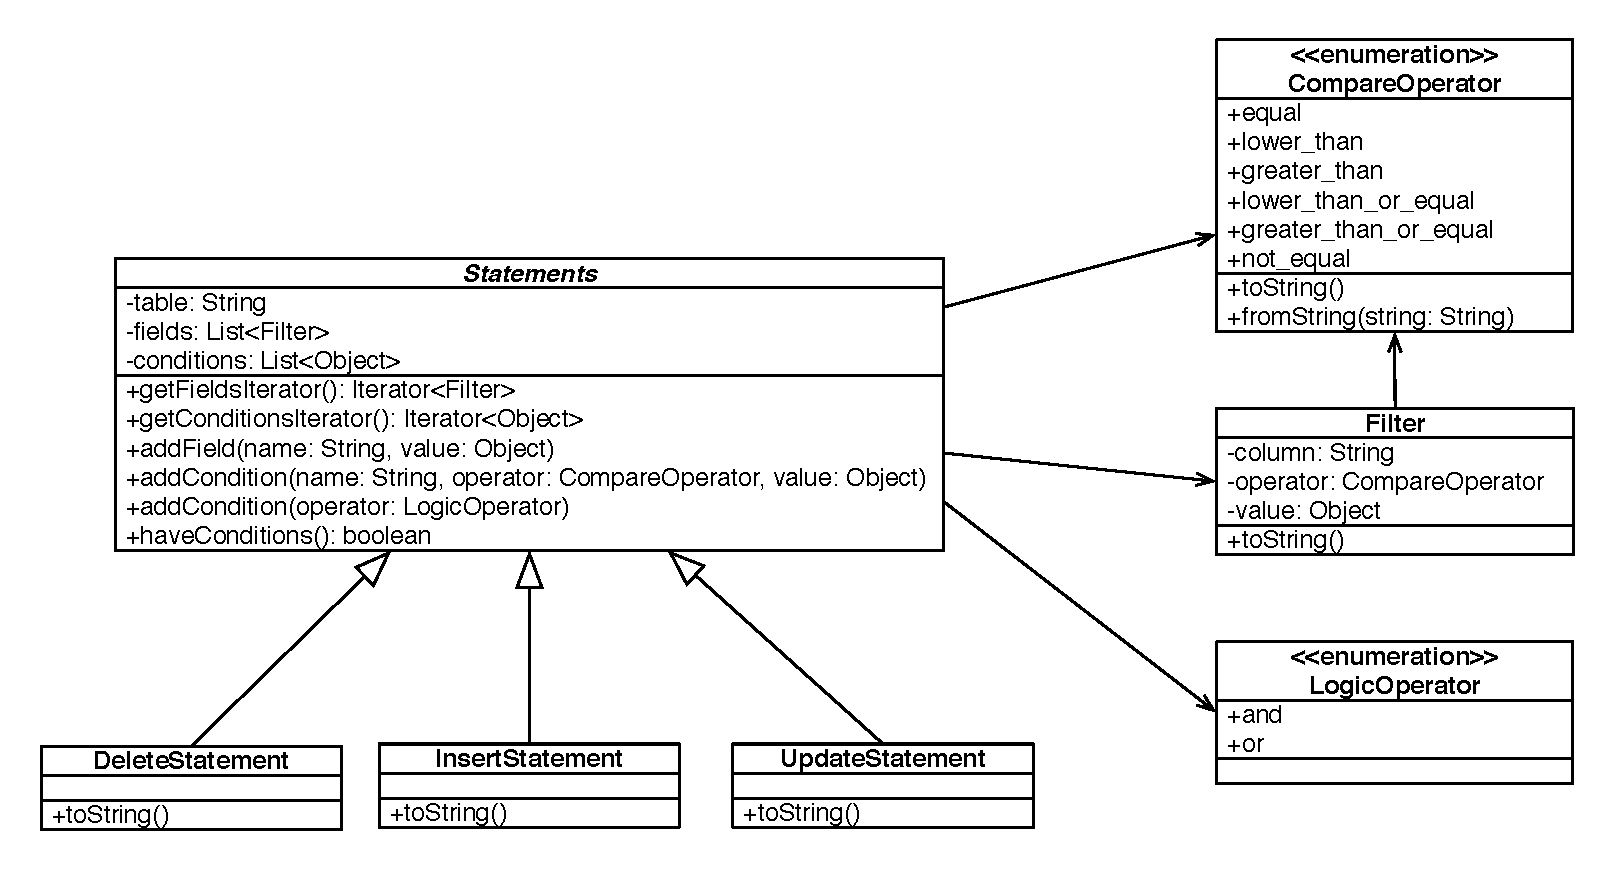
\includegraphics[width=13cm]{images/statements}
  \caption{Statements structure}
  \label{fig:statements}
\end{figure} 

\noindent The \texttt{Statement} class maintains three main fields:
\begin{itemize}
\item \texttt{table}, that contains the table which the statements refer to;
\item \texttt{fields}, maintains a list of elements that represents, in case of an \textit{UPDATE} statements, the the values inside the \textit{SET} clause and, thus, the column names associated with their value; in case of \textit{INSERT} statements, the column names and their value that should be inserted;
\item \texttt{conditions}, a linked list of \texttt{Filter} elements and \texttt{CompareOperator} elements, to represents the \textit{WHERE} clause.
\end{itemize} 

\noindent Since not all those elements are needed in all the statements type, specific statements implementations overrides the method that \texttt{Statements} provide for handling those fields to deny their usage. For example since the \textit{INSERT} statement does not permit a \textit{WHERE} clause, trying to add a condition on that kind of statements will result in an \texttt{UnsupportedOperationException}. Another case is the \textit{DELETE} statements that requires only the \textit{WHERE} clause, so when trying to add a \textit{field} the exception is thrown.

\newparagraph After having defined the statements structure, it is then necessary to provide a way to build the correct instance of a statement, starting by the query or by the operation on an object.
To do this in an agile way, a builder class has been implemented.

\begin{figure}[tbh]
  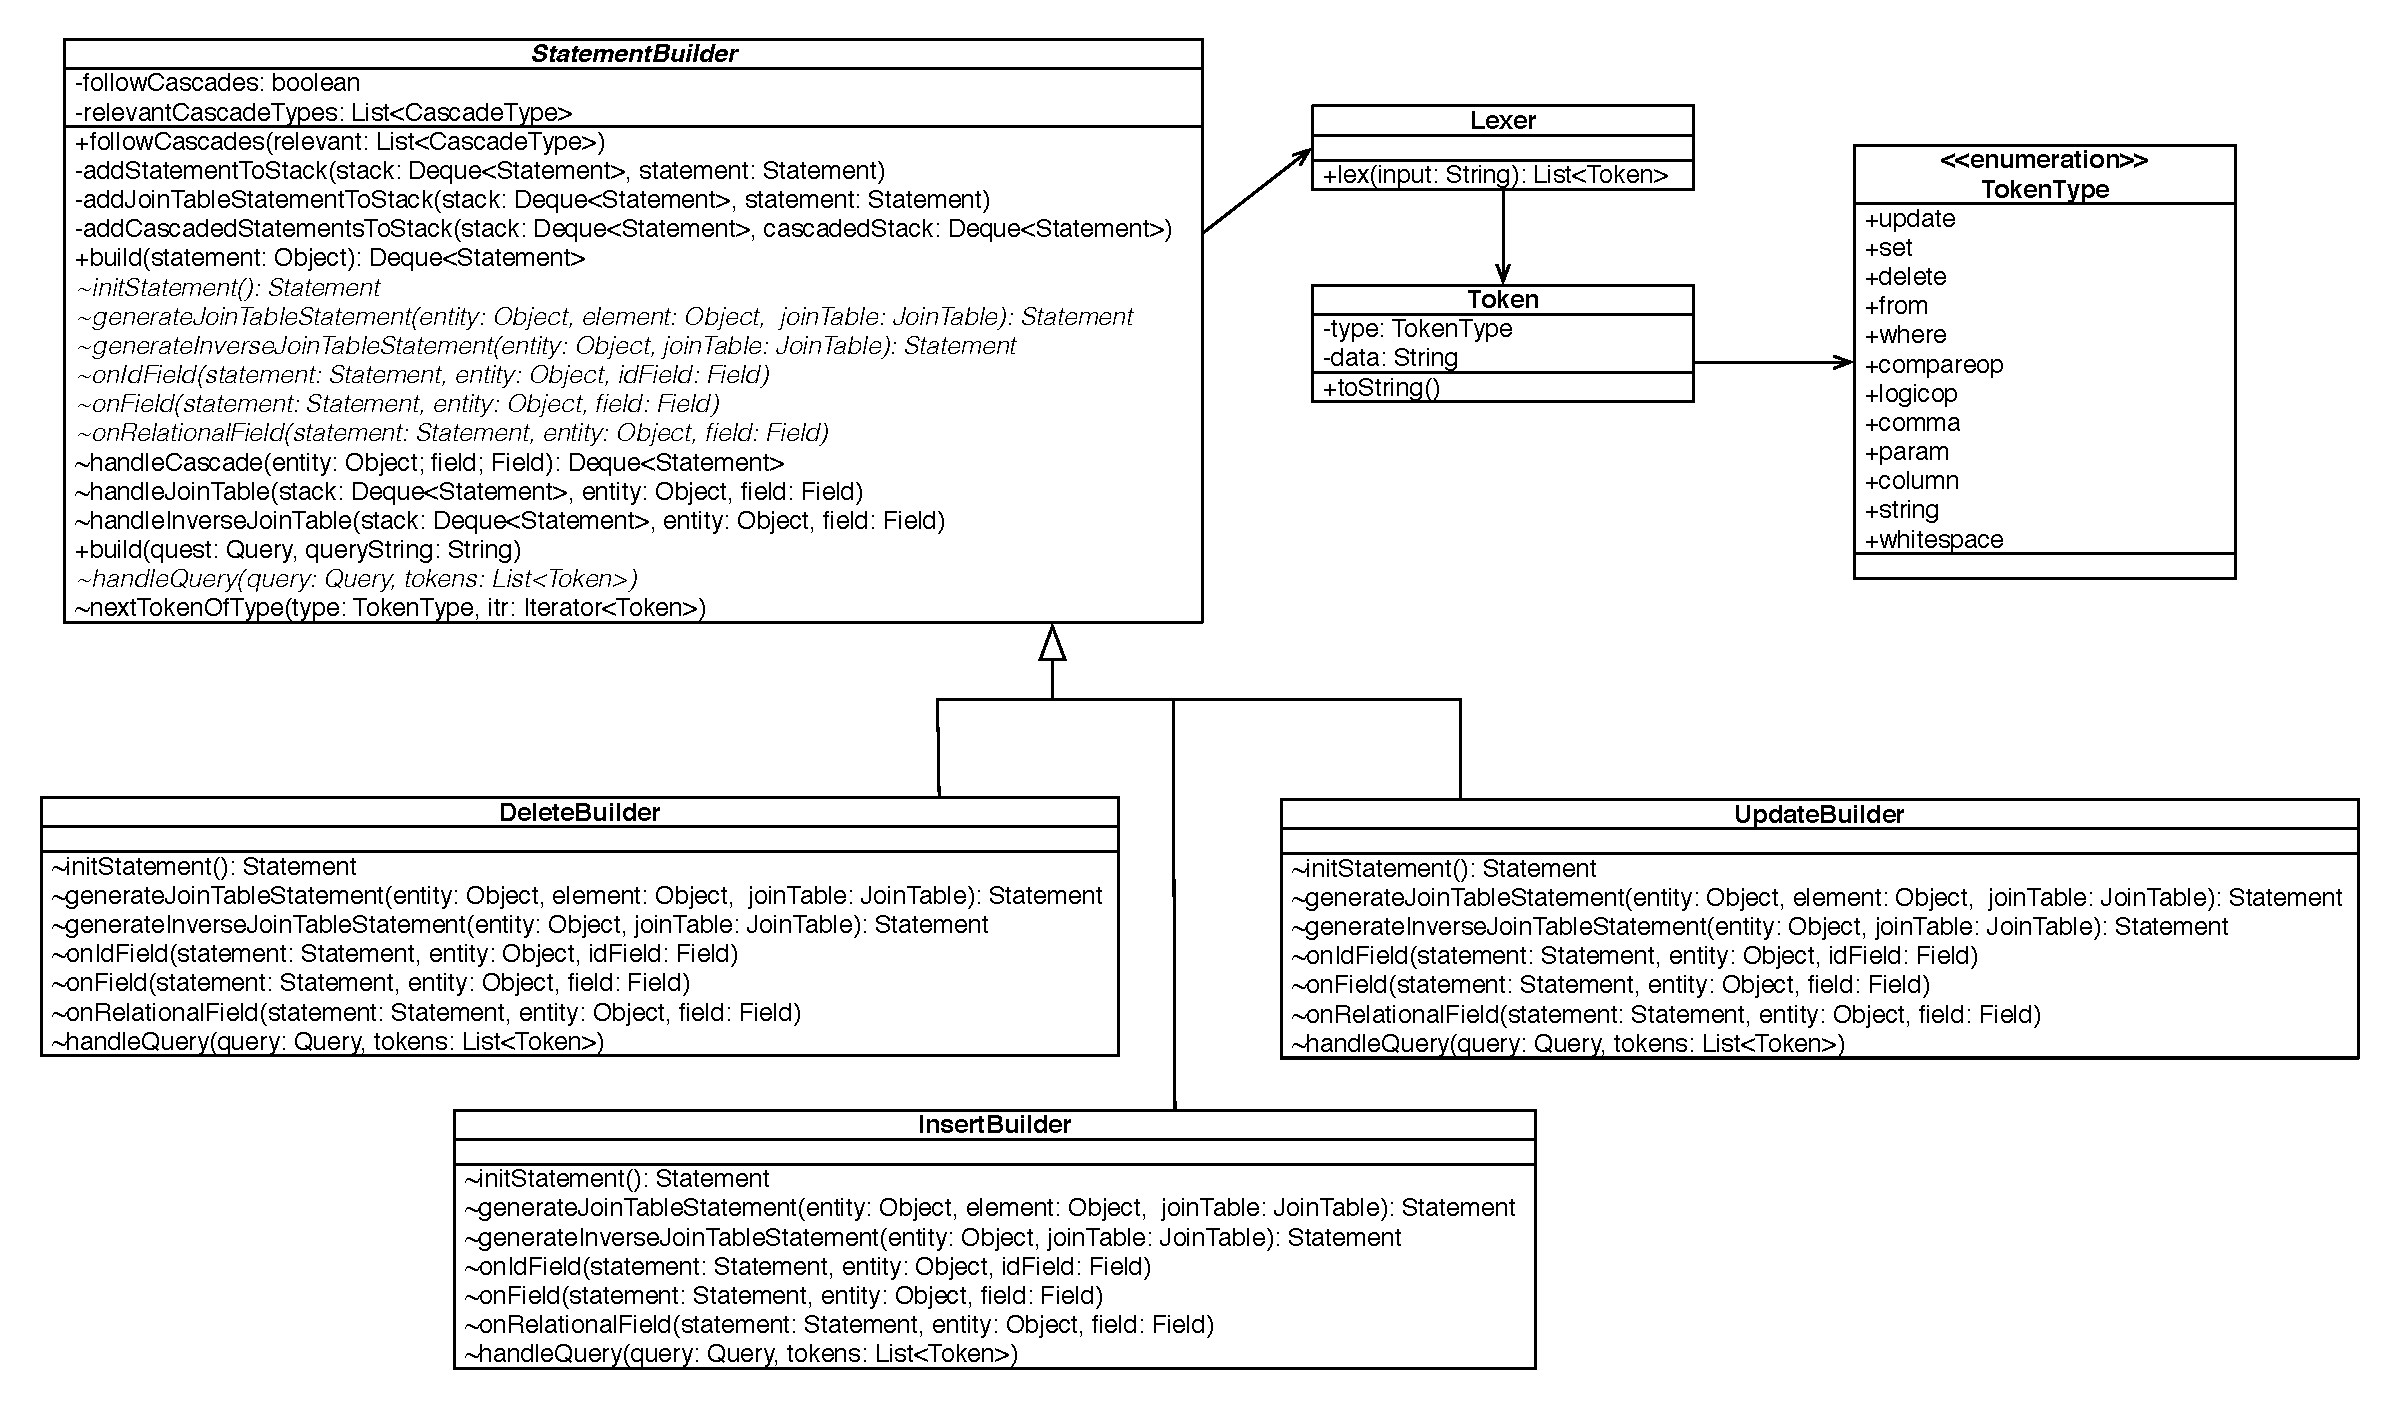
\includegraphics[width=16cm]{images/builders}
  \caption{Statement builders}
  \label{fig:builders}
\end{figure} 

\noindent The class diagram of the builders, shown in figure \ref{fig:builders}, shows that the same pattern used for statements has been adopted.

\noindent The main abstract class \texttt{StatementBuilder} provides the facilities to build a generic statement both from object and from a query string.
Since many operations are the same, for all the three types of statements to be built, the \texttt{StatementBuilder} class provides an implementation of those common behaviors, and it defines some \textit{abstract} methods that are statement-specific and that handled in different ways in the three statement builder classes: \texttt{InsertBuilder}, \texttt{UpdateBuilder} and \texttt{DeleteBuilder}.
This degree of abstraction has been possible due to the abstract definition of the \texttt{Statement} class which allows to the \texttt{StatementBuilder} to act independently from the specific statement type and then to delegate to the specific builder, in the cases in which such abstraction is not sufficient anymore.

\subsection{Build statements from objects}
The main issue in generating statements from objects are the cascade types. From the JPA specification \cite{book:projpa2}, the user, on relational fields, can define which type of cascade type he wants to be applied upon operations on the entity. The cascade type can be specified through the annotation \texttt{@CascadeType}, four are the relevant values:
\begin{itemize}
\item \texttt{PERSIST}, when the entity is persisted, every related entity is persisted too, without the need of any explicit persist for that entity;
\item \texttt{MERGE}, when the entity is updated, every related entity is updated too, without the need of any explicit merge for that entity;
\item \texttt{REMOVE}, when the entity is deleted, every related entity is deleted too, without the need of any explicit delete for that entity;
\item \texttt{ALL}, which enclose all the previous types.
\end{itemize}

\noindent The problem in supporting such operations is that statements generated by cascade must keep a logical order, an example is reported in the code snippet \ref{code:statements-ordering} in which the insert operation for the \texttt{Employee} should happen after the insert of the \texttt{Department} since the employee maintains a foreign key of the department n which he works.

\begin{lstlisting}[language=SQL, caption=Statements ordering example, label=code:statements-ordering]
INSERT INTO Department (id, name) VALUES ('123', 'Computer Science')

INSERT INTO Employee (id, name, department_id) VALUES ('456', 'Fabio', '123')
\end{lstlisting}

\noindent During the development we decided to make the cascade following optional and thus it is configurable in the \textit{migration.xml} file (see the appendix \ref{app:migration} for further details) but also at run-time by calling the appropriate methods on the class \texttt{BuildersConfiguration}. The statements builders, when created, ask to the \texttt{BuildersConfiguration} class in order to decide if the build process should or not consider the cascade types and, if its the case they set the \texttt{relevantCascadeTypes} accordingly.
The relevant cascade types have been defined as follow:
\begin{enumerate}
\item \texttt{ALL} and \texttt{PERSIST}, for \textit{INSERT} statements
\item \texttt{ALL} and \texttt{MERGE}, for \textit{UPDATE} statements
\item \texttt{ALL} and \texttt{REMOVE}, for \textit{DELETE} statements
\end{enumerate}
\noindent The statements execution ordering is the same that should be respected for SQL databases in case foreign key constraints are applied, so, for example, \textit{join table statements} must be taken with particular care since inserts in the join table must happen \textbf{after} the insert of the entity itself and deletes in the join table must happen \textbf{before} the delete of the entity itself. An example is reported in the code snippet \ref{code:join-statements}

\begin{lstlisting}[language=SQL, caption=Join table statements ordering example, label=code:join-statements]
# insert entities
INSERT INTO Employee (id, name) VALUES ('123', 'Fabio')
INSERT INTO Project (id, name) VALUES ('456', 'Apollo')

# insert record in the join table
INSERT INTO Employee_Project (id, employee, project) VALUES ('a', '123', '456')

# deleting the employee
DELETE FROM Employee_Project WHERE id = 'a'
DELETE FROM Employee WHERE id = '123'
\end{lstlisting}

\newparagraph The abstract builder class \texttt{StatementBuilder} provides a single entry point for statements building, by means of the method \texttt{build(Object entity)}. This method is designed following a template pattern, the designed general algorithm (reported in algorithm \ref{code:statements-building}) performs all the operations needed to build the statement, and it calls several methods defined as abstract, which are implemented in the specific builders (since they require specific logic), and several hook methods that can be overrided by the specific builders to change the algorithm behavior.

\begin{algorithm}[h]
  \scriptsize
  \begin{algorithmic}[1]
  \Function{build}{$object$} 
    \State $stack \gets$ empty queue
    \State $cascadedStack \gets$ empty queue
	\State $statemet \gets$ \Call{initStatement}{}
    \State \Call{setTableName}{$statement$, $object$}
    \ForAll{$field \gets$ \Call{getFields}{$statment$}}
      \If{\Call{isRelational}{$field$} $\And$ \Call{ownRelation}{$field$}}
        \If{$handle$\textunderscore $cascades$}
          \State $cascadedStack \gets$ \Call{handleCascade}{$object$, $field$}
        \EndIf
        \If{\Call{isManyToMany}{$field$}}
          \State \Call{handleJoinTable}{$stack$, $entity$, $field$}
        \Else
        	  \State \Call{onRelationalField}{$statement$, $entity$, $field$}
        	\EndIf
      \Else
        \If{\Call{isManyToMany}{$field$}}
          \State \Call{handleInverseJoinTable}{$stack$, $entity$, $field$}
        	\EndIf
      \EndIf
        \If{\Call{isId}{$field$}}
          \State \Call{onIdField}{$statement$, $entity$, $field$}
        \Else
          \State \Call{onField}{$statement$, $entity$, $field$}
        \EndIf
    \EndFor        
    \State \Call {addStatementToStack}{$stack$, $statement$}
    \If{\Call{isId}{$field$}}
      \State \Call{addCascadedStatementsToStack}{$stack$, $cascadedStack$}
    \EndIf
  \EndFunction
  \end{algorithmic}
  \caption{Template algorithm for statements building}
  \label{code:statements-building}
\end{algorithm}

\noindent Cascade generation is handled through the method \texttt{handleCascade(Object entity, Field field)} where \texttt{field} is the field of the entity that represents the related entity. The \texttt{handleCascade} method checks whenever a statements needs to be generated, based on \texttt{relevantCascadeTypes} and then it recursively calls \texttt{build(Object entity)} passing as \texttt{entity} the related object. 

\subsection{Build statements from JPQL queries}
The main problem for JPQL queries is parsing. Since JPQL is an object querying language, it makes use of an object identifier on which it uses the dot notation to specify the object properties, furthermore JPQL allows the user to define parameter placeholders (the ones starting with ":") that are filled later through the method \texttt{setParameter(String name, Object value)} of the \texttt{Query} class.

\noindent The translation that should be performed is shown in the following snippet:

\begin{lstlisting}[language=SQL, caption=JPQL to SQL translation, label=code:query-translation, numbers=none]
# JPQL query string
UPDATE Test t SET t.name = :name WHERE t.salary >= :salary

# SQL version
UPDATE Test SET name = 'Fabio' WHERE salary >= '42'
\end{lstlisting} 

\noindent The mapping among \textit{parameter name} and its \textit{value} is kept in the \texttt{CloudQuery} and \texttt{TypedCloudQuery} classes by intercepting the \texttt{setParameter}.

\newparagraph To solve the parsing problem, the Kundera code was inspected to understand how JPQL queries are parsed, but it turned out they used a custom quite-complex parser, especially for validation purposes. Even looking online no specific JPQL parser has been found so, since we are not interested in validating queries or build complex logic on them, a simple and less time consuming solution was to write a lexer that through regular expressions tokenizes the JPQL string.

\noindent Even the building of statements from queries follows a template pattern, the \texttt{StatementBuilder} class provides the template method \texttt{build(Query query, String queryString)} that tokenizes the query using the lexer and then calls the abstract method \texttt{handleQuery(query, tokens)} that is implemented in \texttt{DeleteBuilder} and in \texttt{UpdateBuilder} which are responsible of iterating over the tokes to build the correct \texttt{Statement} instance.
The \texttt{build(Query query, String queryString)} calls other various hook methods that can be overrided by the specific builders to change the algorithm behavior.

\subsection{Sending statements to Hegira}
Both the method \texttt{propagate(Query query)} and \texttt{propagate(Object entity, OperationType operation)} fill a statement stack which contains the generated statements, in the execution order.

\noindent When iterating over the statement stack, statements are extracted one at a time from the head of the stack (LIFO order). Each of the extracted statement is then sent to \texttt{Hegira}.

%\newparagraph \textbf{TODO update when this part will be done}

\section{Interoperability of stored data}
\label{sec:data-interoperability}
The Kundera client described in chapter \ref{chap:kundera} was developed to be as consistent as possible with the other clients, developed by the Kundera staff, to be more likely accepted by the community and so are not thought to store data in a way other clients can interpret them, and thus are not interoperable.
In an optic of data migration, what we want to achieve is that, data stored within a database, and migrated to another one, are still readable from the application without any changes, besides the new database configuration. 

\noindent The problem for Kundera clients are the relationships. Each database has its own way to define identifier for the persisted entities; for example, in Google Datastore there is the \texttt{Key} with a \textit{Kind} and an \textit{identifier}; for Azure there are the \textit{partition-key} and the \textit{row-key}. These concepts are different, but actually quite similar since both databases are key-value columnar databases. 
A solution to the problem would have been to modify the migration system in order to make it aware of the problem and let it translate the relational columns in the format of the target database; in this way, the relational columns should have been identified in some way to let the system recognize them by adding a pre-defined prefix or a suffix to those columns.
Since this solution requires a good amount of changes in the migration system, other solutions have been explored.
 
\newparagraph Back to the concept of identifier, generally, in columnar databases, columns are grouped in a \textit{column family} and set of columns are identified by a \textit{key}, actually the \textit{key} can span among different \textit{column families}, but that is not the case either in Datastore or Azure Tables.
The pair \textless\textit{column family}, \textit{key}\textgreater
is sufficient to identify an entity (composed by one or more columns), so a mapping is needed between database-specific terminology to the more general one, this mapping is shown in table \ref{table:mapping}.

\begin{table}[h]
\centering
\vspace{1em}
\renewcommand{\arraystretch}{1.4}
\begin{tabular}{lcc}
\hline
\textbf{General concept} & \textbf{Datastore} & \textbf{Azure Table}\\ 
\hline\hline
Column Family & Kind & partition-key \\
\hline
Key & key-identifier & row-key \\
\hline
\end{tabular}
\caption{Column family and Key mapping among supported databases.}
\label{table:mapping}
\end{table}

\noindent At this point we needed a common way of persisting relationships as column family, and key in a way that is interoperable among both the client extension.
The proposed solution is to persist \texttt{columnFamily\textunderscore key}. This solution has to be preferred w.r.t the one that required modification of the migration system since the interoperability is achieved transparently by it.

\subsection{Kundera clients modification}
Since lot of work has already been done on the Kundera clients, the modification to them has been made on a separate branch of the projects named \textit{migration}.

\paragraph{Google Datastore} The Datastore extension has been modified to persist relationships as \texttt{kind\textunderscore key-identifier} instead of the \texttt{Key} instance.
Join tables require particular care, Kundera is not providing the class of the entities involved in the join table, but only the column names and the identifier (the one with the \texttt{@Id} annotation). Queries are possible even if the \textit{Kind} is unknown, since Kundera provides the entity class with the entity identifier as arguments to find operation.
To be more consistent, and to apply the newly defined identifier pattern (\texttt{kind\textunderscore key-identifier}) even for join tables, a map is maintained in the client and built inspecting Kundera meta-data, to keep track of which entity classes are involved in which many to many relationship.

\paragraph{Azure Tables} The Azure Tables extension has been modified too to reflect the newly defined standard for relationships. In Azure Tables relationships were already being saved as \texttt{partition-key\textunderscore row-key} due to the lack of a class similar to \texttt{Key} for Datastore that encapsulate them. The actual problem here is that user can manually handle the partition-key, but it is not a possibility that can be guaranteed anymore since if an entity is persisted as \texttt{partition-key\textunderscore row-key}, the \textit{partition-key} will be interpreted by the Datastore extension as a \textit{Kind}.
Since the \texttt{Kind} in Datastore extension is the entity table name, it has been decided to lock the Azure Table partition-key to the table name, so that the user cannot decide on its own, since this will break the interoperability of data.

\noindent The same discussion for the join tables previously made for Datastore , also applies for the Azure Table extension.

\section{Summary}
In this chapter has been rapidly described the CPIM structure and the architecture of the NoSQL service before this work. Then it has been described how it was possible to integrate Kundera as unique persistence provider in the NoSQL service together wit the problems encountered in the process.

\noindent From section \ref{sec:hegira} has been described the general interaction we wanted to build to make CPIM and Hegira communicate. Then the architecture and the design choices operated in order to develop such interaction, were introduced and described.


%--------------------------------------------------------------------------------
% Evaluation
%--------------------------------------------------------------------------------
\chapter{Evaluation}
\label{chap:eval}
\section{Introduction}
In this chapter, in section \ref{sec:crud} will be discussed the tests used to develop the two Kundera extensions.
In section \ref{sec:performance} will be described the YCSB framework that we have used to test the performance of the developed extensions with respect to the low level API.
Finally in section \ref{sec:data} we present the application developed to test the data synchronization capabilities of CPIM while persisting data through the Datastore Kundera extension. 

\section{Test CRUD operations}
\label{sec:crud}
The Kundera extensions development, due to the lack of information both in the documentation and from the community, has been approached in a test driven way.
The first step was then writing the required JUnit tests for the features we have planned to support.

\newparagraph We primarily want to achieve code portability of model classes, this should be exploited by the usage of the JPA interface but, as stated in chapter \ref{chap:ps}, there were problems in the old NoSQL service implementation relatively to this point.
Secondary we want to be sure that while entities are persisted in the underlying NoSQL database, they can be restored without any loss of information and thus the mapping between entities and the NoSQL database data model behave correctly in both verses.
Hence test the extensions cannot be done directly by testing single methods behavior inside the extensions code, this will for sure test the correctness of the operations but, since Kundera clients are not obliged to follow a rigid structure for their code in the implementation of the required interfaces, tests written for a client are not guaranteed to run correctly for another one. 

\noindent The approach we adopted was to define a single test suite, that will test each one of the feature we planned to support, by interacting directly with Kundera through the JPA interface. This make us able to use the same tests independently of the specific extension and thus testing the correctness of CRUD operations through the JPA interface and the portability of the code by means of tests portability.

\noindent Those tests have been primarily used to test the extensions during the development phase but they have also been executed on the remote databases instances by connecting to them through the network from the development machine. This test has been made to guarantee the correct functioning of the two extensions on real databases instance since tests runned locally are executed  against emulators of real storages.

\subsection{Tests structure}
Tests are composed by the entities, annotated with the JPA annotations, and a test class for each feature.
There are 20 defined entities that includes:
\begin{itemize}
\item simple entities related with the JPA relationships annotations, used to test relationships among entities;
\item embeddable entities and specific entities that uses those embeddable entities as data types, both types used to test the embedded feature;
\item entities with enum fields, used to test the enum fields support;
\item entities declared with different data types for the primary key identifier, used to test ids auto-generation and user-defined ids validation.
\end{itemize}

\noindent The test classes developed for testing the correctness of relationships are:
\begin{itemize}
\item \texttt{MTMTest}, to test the \textit{Many to Many} relationship type;
\item \texttt{MTOTest}, to test the \textit{Many to One} relationship type;
\item \texttt{OTMTest}, to test the \textit{One to Many} relationship type;
\item \texttt{OTOTest}, to test the \textit{One to One} relationship type;
\end{itemize}
\noindent All of those test classes implements two different methods: \texttt{testCRUD()}, that test the relationship by interacting with the method of the \texttt{EntityManager} interface, and \texttt{testQuery()}, that test the relationships by reading, updating and deleting entities through JPQL queries.

\newparagraph The remaining tests classes are:
\begin{itemize}
\item \texttt{ElementCollectionTest}, that tests the JPA feature for persisting list of entities within another one;
\item \texttt{EmbeddedTest}, that tests the JPA feature of persisting user-defined data-types as field of entities;
\item \texttt{EnumeratedTest}, that tests the JPA feature of persisting enum fields;
\item \texttt{QueryTest}, that tests the execution of various \textit{SELECT} queries and the support for the various JPQL clauses in queries.
\end{itemize}

\section{Performance tests}
\label{sec:performance}
We wanted to test the overhead of the developed Kundera extensions with respect to direct use of low-level API. To test those kind of performance in terms of throughput and latency of the read and write operations, we have used Yahoo Cloud Serving Benchmark.
We choose this approach since it was already used by Kundera developers to estimate the overhead that Kundera adds to the low-level API versions of its clients. Hence by using the same method we are able to compare our results to the ones of Kundera.

\subsection{Yahoo Cloud Serving Benchmark}
Yahoo Cloud Serving Benchmark (YCSB) is a framework with the general goal of facilitating performance comparisons of the new generations o cloud serving systems \cite{paper:ycsb}.

\noindent YCSB provides the facility to benchmark various NoSQL database systems such Cassandra, DynamoDB, Voldemort, MongoDB and many others.
The key feature of the benchmark system is extensibility, it in facts supports easy definition of new \textit{workloads} and new systems to benchmark.

\begin{figure}[tbh]
  \centering
  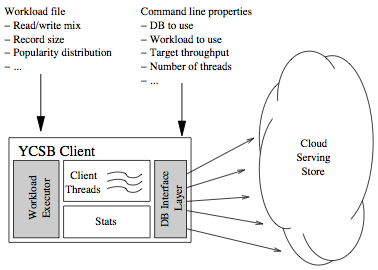
\includegraphics[width=10cm]{images/ycsb_architecture}
  \caption{YCSB architecture \cite{paper:ycsb}}
  \label{fig:ycsb-architecture}
\end{figure} 

\newparagraph The access point to the benchmark framework is the \textit{YCSB Client} which is responsible of generating the operations which make up the workload. The workload is then executed by the \textit{Workload executor} that drives multiple client threads which in turn execute a sequential series of operations by making calls to the \textit{database interface layer}.
The workloads are executed in two separate phases:
\begin{enumerate}
\item the \textbf{load phase}, which loads the workload data to the datastore instance;
\item the \textbf{transaction phase}, which execute the workload on the loaded data.
\end{enumerate}
\noindent Each thread rules the rate at which it generate requests ad measure the latency and the throughput of its operation. At the end of the benchmark, the statistics modules aggregates the measurements and build the report.

\subsection{YCSB adapters}
The YCSB Client abstracts from the specific database system under test through the \textit{database interface layer}. This allows YCSB to generate operations like ``read record'' or ``update record'' without having to understand the specific API of the underlying database. The  \textit{database interface layer} is a simple abstract class that provides read, insert, update, delete and scan operations. 
\noindent To create a database adapter the abstract class \texttt{com.yahoo.ycsb.DB} must be extended and the following methods needs to be implemented:
\begin{itemize}
\item \texttt{init()}, which is used to perform any initialization operation such as connecting to the database instance and is called once per thread;
\item \texttt{read(String table, String key, ...)}, which is supposed to read a single record;
\item \texttt{scan(String table, String startkey, int recordcount, ...)}, which is supposed to perform a range scan;
\item \texttt{insert(String table, String key, ...)}, which is supposed to update a single record;
\item \texttt{delete(String table, String key)}, which is supposed to delete a record.
\end{itemize}

\newparagraph To be able to compare the benchmarks result to the Kundera ones, we developed  several YCSB adapters:
\begin{itemize}
\item an adapter for Google Datastore low-level API
\item an adapter for Google Datastore through the developed Kundera extension
\item an adapter for Azure Tables low-level API
\item an adapter for Azure Tables through the developed Kundera extension
\end{itemize}
\noindent Even if the adapters for Hbase were already been developed by Kundera, they have been both re-written. The Kundera client adapter were re-written to be identical to the ones for Google Datastore and Azure Tables; the low-level API version were re-written because the Kundera client for Hbase has been updated to supported the latest version of the software but the YCSB adapter was not.

\subsubsection{Kundera adapters}
For the Kundera version of the adapters the same structure has been kept for all three databases. The \texttt{EntityManagerFactory} is instantiated at the adapter construction since this operation causes Kundera to initialize all its internal structure; an instance of the entity manager is instead created in the \texttt{init} method since the initialization of the \texttt{EntityManager} causes the initialization of the specific Kundera client, in this way each thread will have its own \texttt{EntityManager} with which interact and the same overhead with regards to database connection operation.
Apart from the \texttt{scan} method, which was not implemented, every other operations calls the responsible method on the \texttt{EntityManager}, in the code \ref{code:insert-operation} is shown an example for the insert operation.

\begin{lstlisting}[language=Java, caption=Insert operation of the Azure Tables adapter, label=code:insert-operation]
@Override
public int insert(String table, String key, ...) {
    ...
    try {
        AzureTableUser user = new AzureTableUser(key, nextString(),, ...);
        em.persist(user);
        if (timeToClearEntityManager()) {
            em.clear();
        }
        return OK;
    } catch (Exception e) {
        return ERROR;
    }
}
\end{lstlisting}

\noindent In the code \ref{code:insert-operation} there are two elements that are worth deep explanation. The first thing to notice is that is persisted an instance of \texttt{AzureTableUser} in fact we were not able to persist the entities generated by YCSB because, to be able to persist an entity with the JPA, we need an annotated class which is then listed in the \textit{persistence.xml}. For this reasons three different user class and three different persistence units has been defined:
\begin{itemize}
\item \texttt{AzureTableUser}, which refer to \texttt{kundera\textunderscore azure\textunderscore pu}, the persistence unit with the configuration for Azure Tables;
\item \texttt{DatastoreUser}, which refer to \texttt{kundera\textunderscore datastore\textunderscore pu}, the persistence unit with the configuration for Google Datastore;
\item \texttt{HBaseUser}, which refer to \texttt{kundera\textunderscore hbase\textunderscore pu}, the persistence unit with the configuration for Hbase.
\end{itemize} 
\noindent The second thing to notice is the call to the \texttt{timeToClearEntityManager()} method, which checks, with respect to an internal counter, if has been persisted 500 entities, if this is the case the persistence cache is cleared by calling \texttt{EntityManager.clear()}. If this operation is not performed, entities read can occur within the persistence cache bypassing the request to the underling database. We choose to clear the cache every 500 entities in our workloads of 100.000 entities, to maintains the same proportion with the one used by Kundera in their test in which they clear the entity manager every 5.000 entities on workloads of 1 million operations.

\subsubsection{Low-level API adapters}
Also the adapters for the low-level API version follows the same general structure. The connection to the database is performed, through low-level API in the \texttt{init} method, to have a common behavior with respect to the Kundera adapters; read, insert and delete operations are performed by a call to the low-level API, while the \texttt{scan} method has not been implemented.

\noindent The \texttt{init} method uses the properties defined in the property filesm specified in the execution command of the benchmark, to locate the remote database and instantiate a connection.

\subsection{YCSB tests}
YCSB comes with a core set of workloads, each workloads represents a particular mix of read and write operations and define the total number of operations that should be executed. 
\noindent YCSB benchmarks are executed in two separate phases and each of them generates a report. From the report of the \textit{load} phase, since this phase is responsible of storing the data required to run the workload to the target database, we obtains information about the throughput and the latency for the write operation; from the \textit{transaction} phase we want to obtain information about throughput and latency for the read operation. To do this we run a custom workload composed of 100.000 operations entirely of type read so that the \textit{transaction} phase will generates the statistics we need.
\noindent Defined the adapters and the workload we were able to execute the tests.

\subsubsection{Google Datastore tests}
The tests for Google Datastore has been executed over a remote Datastore instance in an application billed by Politecnico di Milano and configured to accept remote API execution.

\noindent The results of the tests are reported in figure \ref{fig:gae-test-read} for the read operation and in figure \ref{fig:gae-test-write} for the write operation.
 
\begin{figure}[tbh]
  \centering
  \subfloat[Throughput]{
    
\includegraphics[width=5cm]{images/logopm}
  }
  \qquad
  \subfloat[Latency]{
    
\includegraphics[width=5cm]{images/logopm}
  }
  \caption{Google Datastore - read operation benchmark results}
  \label{fig:gae-test-read}
\end{figure} 

\begin{figure}[tbh]
  \centering
  \subfloat[Throughput]{
    
\includegraphics[width=5cm]{images/logopm}
  }
  \qquad
  \subfloat[Latency]{
    
\includegraphics[width=5cm]{images/logopm}
  }
  \caption{Google Datastore - write operation benchmark results}
  \label{fig:gae-test-write}
\end{figure} 
 
\subsubsection{Azure Tables tests}
The tests for Azure Tables has been executed over a remote storage instance deployed in Azure from the billing account of Politecnico di Milano.

\noindent The results of the tests are reported in figure \ref{fig:azure-test-read} for the read operation and in figure \ref{fig:azure-test-write} for the write operation.
 
\begin{figure}[tbh]
  \centering
  \subfloat[Throughput]{
    
\includegraphics[width=5cm]{images/logopm}
  }
  \qquad
  \subfloat[Latency]{
    
\includegraphics[width=5cm]{images/logopm}
  }
  \caption{Azure Tables - read operation benchmark results}
  \label{fig:azure-test-read}
\end{figure} 

\begin{figure}[tbh]
  \centering
  \subfloat[Throughput]{
    
\includegraphics[width=5cm]{images/logopm}
  }
  \qquad
  \subfloat[Latency]{
    
\includegraphics[width=5cm]{images/logopm}
  }
  \caption{Azure Tables - write operation benchmark results}
  \label{fig:azure-test-write}
\end{figure} 

\subsubsection{Hbase tests}
Hbase test should have been executed over an instance of Hbase, in full distributed configuration, in the cloud of Politecnico di Milano but due to a failure of the host machines the tests cannot be performed.

\noindent In figure \ref{fig:hbase-test-read} and \ref{fig:hbase-test-write} are reported the results obtained while testing the Hbase adapters. They have been executed on a workload of 1.000 entities in a locally installed instance of Hbase.

\begin{figure}[tbh]
  \centering
  \subfloat[Throughput]{
    
\includegraphics[width=5cm]{images/logopm}
  }
  \qquad
  \subfloat[Latency]{
    
\includegraphics[width=5cm]{images/logopm}
  }
  \caption{Hbase - read operation benchmark results}
  \label{fig:hbase-test-read}
\end{figure} 

\begin{figure}[tbh]
  \centering
  \subfloat[Throughput]{
    
\includegraphics[width=5cm]{images/logopm}
  }
  \qquad
  \subfloat[Latency]{
    
\includegraphics[width=5cm]{images/logopm}
  }
  \caption{Hbase - write operation benchmark results}
  \label{fig:hbase-test-write}
\end{figure} 

\subsection{Discussion}
The main objective of our tests was to guarantee that the loss of performance, between the Kundera version of the client and the client written with direct use of the low-level API, was minimum.

\noindent The objective was also to compare our results with the results obtained by Kundera with the other client extensions. Since Kundera executed the tests on databases instance that reside on the testing machine we cannot compare our results, in fact, is meaningless to execute the tests for Google Datastore and Azure Table on the storage emulator installed on a development machine. What we decide to do to has been to test the performance of the newly developed client extensions remotely and thus testing on a real instance of the databases on the cloud but, to be able to compare the results with the Kundera ones, we decided also to replicate the test for Hbase on a instance in the cloud infrastructure of Politecnico di Milano.
Moreover, Kundera tests were quite out-dated since they has been executed on version 2.6 of the clients while as, we write, the latest version is the 2.16.

\newparagraph Apart from the comparison with the Kundera results that cannot be done due to the problem in having a functioning Hbase cluster in the Politecnico di Milano cloud, the tests shows that the performance loss due to the Kundera overhead is minimum or at least acceptable given the advantages that Kundera offer in hiding the NoSQL complexity to the user.
As regards the throughput, can be noticed that the Hbase test done locally over 1.000 entities have a considerably lager value with respect to the throughput of the Google Datastore and Azure Tables tests. This is due to two reasons; the first one is that YCSB benchmarks run until the target database reach saturation and thus tries to estimate the maximum possible throughput, the second reason is due to the fact that, while running remotely, the databases instances are addressed through TCP requests and thus the number of connections that the testing system has to handle becomes the bottleneck. 

\noindent Running the tests with less entities will increase the throughput as the number of connection that needs to be maintained open is significantly lower.
As an evidence of this are reported in figure \ref{fig:gae-1000} and \ref{fig:azure-1000} the results of a test run on the same remote instances but with just 1.000 entities.   

\begin{figure}[tbh]
  \centering
  \subfloat[Write throughput]{
    
\includegraphics[width=5cm]{images/logopm}
  }
  \qquad
  \subfloat[Read throughput]{
    
\includegraphics[width=5cm]{images/logopm}
  }
  \caption{Google Datastore - 1.000 entities benchmark results}
  \label{fig:gae-1000}
\end{figure} 

\begin{figure}[tbh]
  \centering
  \subfloat[Write throughput]{
    
\includegraphics[width=5cm]{images/logopm}
  }
  \qquad
  \subfloat[Read throughput]{
    
\includegraphics[width=5cm]{images/logopm}
  }
  \caption{Azure Tables - 1.000 entities benchmark results}
  \label{fig:azure-1000}
\end{figure} 

\section{Hegira generator}
\label{sec:data}
To be able to test the interaction between the CPIM library and the synchronization system and to provide an example of usage of the extended CPIM library, we have developed \textit{Hegira generator}.

\noindent The application provides two behaviors through command line interface, a \texttt{clean} command to clean-up the remote Datastore instance by deleting all the entities of all Kinds, and a \texttt{generate} command that take as argument the number of entities to be generated per table and generates them.

\newparagraph Data generation is done upon a pre-defined entity model inside the application and described by the ER diagram of figure \ref{fig:hegira-generator-er}.
Build an entity generator agnostic to the entities model was not our goal and it would have required a way to automatically build the dependency graph of the entities since entities related to other ones should have a reference to the entity they depends on. Hence the application is aware of the entities dependencies and generates them accordingly.

\begin{figure}[tbh]
  \centering
  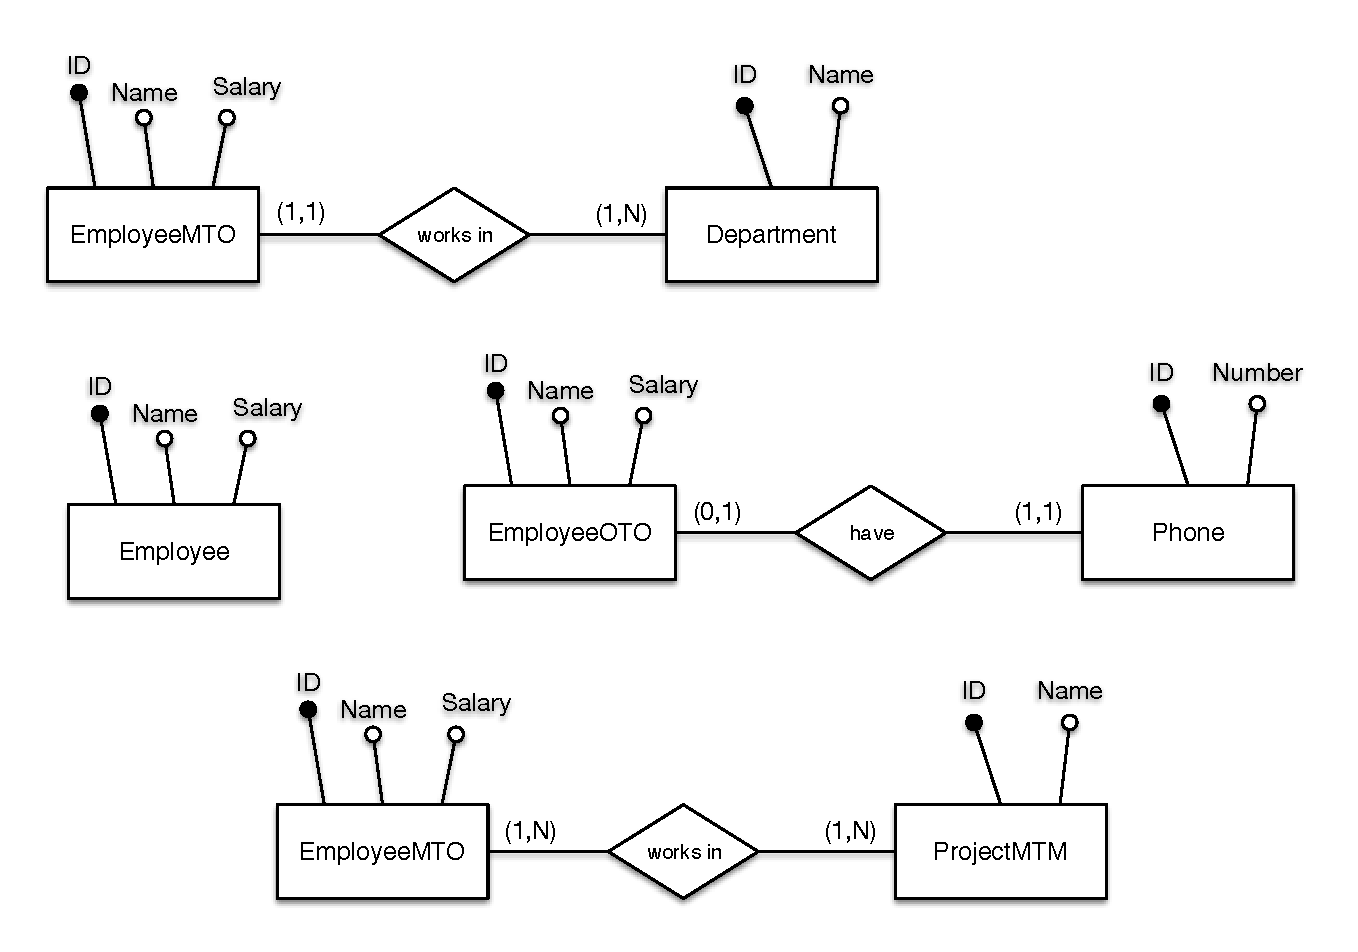
\includegraphics[width=10cm]{images/hegira_generator_er}
  \caption{ER diagram of Hegira-generator model}
  \label{fig:hegira-generator-er}
\end{figure} 

\noindent To be able to generate random entities, two methods are used:
\begin{itemize}
\item \texttt{persist(Class master)} that generates and persist entities without dependencies (such as \texttt{Employee} in the application model;
\item \texttt{persist(Class master, Class slave, DependencyType type)} that generates and persist the entities of the \textit{master} class, then uses randomly extracted entities among those just generated to fill the dependencies for the entities of the \textit{slave} class.
The \texttt{DependencyType} would be \texttt{SINGLE}, if the \textit{slave} class needs just one element to fill the dependency (which is the case of \textit{One to One} and \textit{Many to One} relationships), or \texttt{COLLECTION}, if the \textit{slave} class needs more than one element to fill the dependency (which is the case for \textit{Many to Many} relationships).
\end{itemize}

\noindent The actual entity generation is delegated to the entity itself through reflection since each entity of the model implements the \texttt{Randomizable} interface.
An example of entity genearion through this interface is shown in the snippet \ref{code:randomizable}.

\begin{lstlisting}[language=Java, caption=Entities generation, label=code:randomizable]
@Entity
public class EmployeeOTO implements Randomizable<EmployeeOTO, Phone> {
    ...
    @Override
    public EmployeeOTO randomize(Phone dependency) {
        setName(RandomUtils.randomString());
        setSalary(RandomUtils.randomLong());
        setPhone(dependency);
        return this;
    }
}
\end{lstlisting}
 
\subsection{Exploited CPIM features}
To perform the persist operation of the generated entities is used the \texttt{EntityManager} interface on which is called the \texttt{persist} method, this is completely JPA compliant and the user is not aware of what is done under the hood since communication with the synchronization system is handled automatically. An example is provided in the code \ref{code:example-persist}.

\begin{lstlisting}[language=Java, caption=Persisting entities in CPIM, label=code:example-persist]
CloudEntityManager em = MF.getFactory().getEntityManager();
Department dep = new Department("Computer Science")
em.persist(dep)
\end{lstlisting}

\noindent The persist operation through \texttt{CloudEntityManager} contacts the synchronization system to get the assigned sequence numbers for the specific tables and assign the first of them to the entity before delegating to Kundera the persist operation.

\newparagraph The application make use of the possibility of modifying at run-time the size of sequence numbers range that is requested to the synchronization system. Hence before the persist operation, the size of the sequence number range is set to the double of the number of entities to be generated. This is done through a call to \texttt{SeqNumberProvider.getInstance().setOffset(tableName, offset)}, if the resulting range size is grater than the maximum size that can be requested, is limited to that value. 

\newparagraph the last feature that is exploited by the application is the sequence number backup to file. The backup is configured in the \texttt{migration.xml} file as described in the appendix \ref{app:migration}.
This permit to the application, when is restarted, to restore the sequence numbers without the need of contacting the synchronization system.

\noindent Furthermore, to avoid execution of persist operations on a table which entities generation was completed in a previous execution, a file with the list of the table completely generated is kept in the same folder specified for the sequence numbers backup files.

\section{Summary}
In this chapter we have presented the test of correctness and performance made for the two developed Kundera extension showing the minimal performance loss that Kundera add to the low-level API.
Finally we have presented \textit{Hegira-generator}, the application developed to test the mechanisms developed inside CPIM to interacts with the synchronization system.


%--------------------------------------------------------------------------------
% Conclusions and future works
%--------------------------------------------------------------------------------
\chapter{Conclusions and future Works}
\label{chap:conclusions}
This work presented an approach of interacting with many different NoSQL databases through the CPIM library and the integration of the migration and synchronization system \textit{Hegira}.

\newparagraph The CPIM library has been modified in order to get rid of the previous implementation of the NoSQL service that was not able to guarantee full portability of the application code due to the numerous JPA implementation used to support different NoSQL databases. This work have made order in the CPIM library and added the ability for the users to interact with numerous different NoSQL solution through a common interface, identified in the JPA interface, thanks to Kundera, an open source JPA compliant ORM for NoSQL databases.

\noindent Furthermore have been produced two brand new clients for Kundera contributing thus to the project by adding the support for Google Datastore and Azure Tables. In chapter \ref{chap:eval}, the developed extensions has been tested in terms of throughput and latency in order to verify that the overhead added by Kundera and by its clients was not destructive for performance with respect to the use of low level API for interacting with the NoSQL databases.

\noindent The results showed that, since no significant overhead is added to the low level API version of NoSQLs, the approach we propose is worth the little loss of performance due to the benefit it brings in terms of code portability, through the CPIM library, and the ability of interacting with many different NoSQL databases with a unique and well known interface.

\newparagraph\newparagraph The NoSQL service of CPIM library has been further modified to integrate the required logic for interacting with the migration and synchronization system \textit{Hegira}, the work is described in chapter \ref{chap:cpim}. This mitigates the vendor lock-in problem by giving to the user the ability to change the adopted NoSQL technology and still be able to read the migrated data without the necessity of re-engineer the application.
 
\newparagraph Possible future works should continue on both CPIM and Kundera. Indeed, CPIM needs to be updated to interacts with the latest version of the various cloud provider API and some components needs to be rewritten, as explained in section \ref{sec:cpim-problems} for the Queue service.

\noindent Further work can also be done in intercepting the user queries, that are then sent to the migration system, supporting for example the \textit{criteria API} discussed in section \ref{sec:cpim-intercept-queries}.

\noindent Some work can be made in solving the problems that have prevented us from replicating the YCSB tests for Hbase. In this way the results presented in this work can be compared with the results of the tests performed by the Kundera team on the other clients.

\noindent Finally some work can be done in adding to Kundera the support for more NoSQL databases such as Dynamo DB.


%--------------------------------------------------------------------------------
% appendices
%--------------------------------------------------------------------------------
\part*{Appendices\label{part:app}\addcontentsline{toc}{part}{Appendices}}
\appendix
\chapter{Configuring Kundera extensions}
\label{app:kconfig}
\section{Introduction}
Introduzione agli argomenti trattati nell'appendice, dalle 4 alle 10 righe.

\section{\dots}
Argomenti trattati suddivisi sezione per sezione. 
Alla fine del capitolo non includere alcun sommario.



\chapter{Configuring CPIM migration}
\label{app:migration}
\section{Introduction}
Introduzione agli argomenti trattati nell'appendice, dalle 4 alle 10 righe.

\section{\textit{migration.xml}}


\chapter{Run YCSB tests}
\label{app:ycsb}
\section{Introduction}
Introduzione agli argomenti trattati nell'appendice, dalle 4 alle 10 righe.


%--------------------------------------------------------------------------------
% bibliography
%--------------------------------------------------------------------------------
\bibliographystyle{plain}
\bibliography{thesis.bib}

\end{document}
